%%%%%%%%%%%%%%%%%%%%%%% file template.tex %%%%%%%%%%%%%%%%%%%%%%%%%
%
% This is a general template file for the LaTeX package SVJour
% for Springer journals.          Springer Heidelberg 2010/09/16
%
% Copy it to a new file with a new name and use it as the basis
% for your article. Delete % signs as needed.
%
% This template includes a few options for different layouts and
% content for various journals. Please consult a previous issue of
% your journal as needed.
%
%%%%%%%%%%%%%%%%%%%%%%%%%%%%%%%%%%%%%%%%%%%%%%%%%%%%%%%%%%%%%%%%%%%
%
% First comes an example EPS file -- just ignore it and
% proceed on the \documentclass line
% your LaTeX will extract the file if required
\begin{filecontents*}{example.eps}
%!PS-Adobe-3.0 EPSF-3.0
%%BoundingBox: 19 19 221 221
%%CreationDate: Mon Sep 29 1997
%%Creator: programmed by hand (JK)
%%EndComments
  
gsave
newpath
  20 20 moveto
  20 220 lineto
  220 220 lineto
  220 20 lineto
closepath
2 setlinewidth
gsave
  .4 setgray fill
grestore
stroke
grestore
\end{filecontents*}
%
\RequirePackage{fix-cm}
%
%\documentclass{svjour3}                     % onecolumn (standard format)
%\documentclass[smallcondensed]{svjour3}     % onecolumn (ditto)
%\documentclass[smallextended]{svjour3}       % onecolumn (second format)
\documentclass[twocolumn]{svjour3}          % twocolumn
%
% flush right qed marks, e.g. at end of proof
\smartqed

\usepackage[lofdepth,lotdepth]{subfig}
\usepackage{graphicx}
\usepackage{subcaption}
\usepackage{subfigure} % subfiguras
%
\usepackage{mathptmx}      % use Times fonts if available on your TeX system
%
% insert here the call for the packages your document requires
\usepackage{amssymb}
\usepackage{amsmath}
\usepackage{amsfonts}
\usepackage{epstopdf}
\usepackage{mathrsfs} % para formato de letra
\usepackage{hyperref}
\usepackage{enumitem}
\usepackage{array}
\usepackage{tabularx}
\usepackage{supertabular}
\usepackage{fancyhdr}
\usepackage{multirow}
\usepackage{color}
\usepackage{makeidx}
\usepackage{xstring}
\usepackage{setspace}
\usepackage{epsfig}

\usepackage{pgf}
% \usepgfplotslibrary{external} 
% \tikzexternalize

%\usepackage{subfigure}
\usepackage{preview}
% Packages to write pseudo-algorithms %
\usepackage{algorithm}
\usepackage{algorithmic}

% Tikz
\usepackage{stanli}
\usepackage[ugly]{units}
% \usetikzlibrary{decorations}
% \usetikzlibrary{arrows}
\usetikzlibrary{plotmarks}

\usetikzlibrary{%
    decorations.pathreplacing,%
    decorations.pathmorphing%
}

%\usepackage{latexsym}
% etc.

%

% Matrix and vector nodes
\newcommand{\Matrix}[1]{
  \ensuremath{\mathbf{{#1}}}
}
\newcommand{\Vector}[1]{
  \ensuremath{\mathbf{{#1}}}
}

% Divergence
\newcommand{\Div}[1]{
  \ensuremath{div({#1})}
}
% Gradient
\newcommand\Grad[1]{grad({#1})}
\newcommand\GradS[1]{grad^s({#1})}
\newcommand\GradT[1]{grad^T({#1})}


% Partial derivative
\newcommand{\Deriv}[3][]{
  \ensuremath{\frac{\partial^{#1}{#2}}{ \partial {#3}^{#1} }}
}

% Integral
\newcommand{\Integral}[2]{
  \IfStrEqCase{#1}{
    {2}{\ensuremath{\int_{\varGamma_d}{#2}\ d\varGamma}}
    {3}{\ensuremath{\int_{\varOmega}{#2}\ d\varOmega}}
  }
}

%
% Insert the name of "your journal" with
\journalname{Computational Particle Mechanics}
%
\begin{document}

% \title{Novel improvements in the Material Point Method to face
%   dynamic problems: 
%   Local-maximum entropy approximation and an explicit predictor-corrector scheme. \thanks{Funding: This
%     study was funded by Agustín de Betancourt Foundation (grant number
%     262390106114).}
% }

\title{Enhanced Material Point Method to face
  dynamic problems:\thanks{Funding: This
    study was funded by Agustín de Betancourt Foundation (grant number
    262390106114).}
}
\subtitle{Local-maximum entropy approximation and explicit
  predictor-corrector scheme}

\titlerunning{Novel improvements in the Material Point Method to face
  dynamic problems.} % if too long for running head

\author{Miguel Molinos \and
  Pedro Navas \and
  Manuel Pastor \and
  Miguel Martín Stickle
}

%\authorrunning{Short form of author list} % if too long for running head

% \institute{Miguel Molinos \at
%   E.T.S de Ingenieros de Caminos, Canales y Puertos. \\
%   Universidad Politéctnica de Madrid, 28040 Madrid, Spain \\
%   \email{m.molinos@alumnos.upm.es}
%   % \emph{Present address:} of F. Author  %  if needed
%   \and
%   Pedro Navas 
%   \and
%   Manuel Pastor
%   \and
%   Miguel Martín Stickle
% }
% \institute{Miguel Molinos, Pedro Navas and Manuel Pastor \at E.T.S
%   de Ingenieros de Caminos, Canales y Puertos, Universidad Politéctnica de Madrid, 28040 Madrid, Spain, \; \email{m.molinos@outlook.es, pedro.navas@upm.es, manuel.pastor@upm.es}
% }


\date{Received: date / Accepted: date}
% The correct dates will be entered by the editor

\maketitle
\begin{abstract}
  Material Point Method (MPM) has arisen in the recent years as an
  alternative to Finite Element Method (FEM) under the large
  deformation regime. However, the simulation of shock waves
  propagation and other high frequency problems is still challenging
  under this approach due the incapability of the standard MPM time
  integration scheme to filter spurious noises. To overcome this
  limitation in this paper, an explicit predictor-corrector time integration
  scheme has been proposed. Its superior performance mitigates the
  presence of spurious oscillations with minimal dissipation in high
  frequency problems. Other source of numerical noise in MPM 
  occurs when to material points cross computational grid
  boundaries and motivated due to the lack of smoothness of the interpolation
  functions. This noise results in spurious local variations at the material
  points, where strain-stress fields are computed. This could invalidate
  the solution in one case, or damage it in another. To overcome it,
  this document adopts the \textit{local maximum-entropy approximation
    schemes} (LME) a robust substitute for the wide range of shape
  function in MPM. Local \textit{max-ent} approximation may be regarded as a
  \textit{thermalization} of Delaunay triangulation which resolves the
  degenerate cases resulting from the lack or uniqueness of the
  triangulation. Furthermore, by modifying a regularization parameter they
  are able to behave finite element like or as a mesh-free
  method. This capability allows to face a wide range of physics
  with a single shape function family. Finally this paper demonstrates
  the performance of both improvements thorough numerical examples.    
  \keywords{LME \and MPM \and Explicit predictor-corrector \and Dynamic problems}
  % \PACS{PACS code1 \and PACS code2 \and more}
  % \subclass{MSC code1 \and MSC code2 \and more}
\end{abstract}

\section{Introduction}
\label{intro}
Since the proposal of MPM by Sulsky {\it  et al.}
(1994)~\cite{Sulsky1994} as a generalization to solids of the Fluid
Implicit Particle (FLIP) method~\cite{Brackbill1986}. It popularity
has increased due to its ability to deal with large strain regime
without suffer mesh distortion inaccuracies.

However, this method suffers other kind of instabilities, such those
when material points crossing cell boundaries. This give rise to the
development of other interpolation techniques to overcome this
limitation such as the generalized interpolation material point method
(GIMP) Bardenhagen \& Kober (2004)~\cite{Bardenhagen2004}, which has
demonstrate to have a good performance in the finite deformation
regime. However, in the absence of a regular grid, construction of the
weighting functions is only achieved at considerable effort and
computational cost.  Furthermore, as it is  a voxel based
discretization technique, it is prone to suffer voxel domains overlap
or gaps when the material point mesh becomes irregular, which can
introduce severe inaccuracies as noticed Steffen {\it et al.}
(2008)\cite{Steffen2008}. This is similar to the difficulty
encountered by the finite element methods due to element distortion.
A more robust alternative is the dual domain material point method
(DDMP) proposed by Zhang {\it et al.}
(2011)~\cite{Zhang2011a}. Unfortunately this method shows an
unsatisfactory behaviour when particle/cell ratio
decreases~\cite{DHAKAL2016301}, therefore DDMP requires a large number
of particles needed for convergence, this
makes the method very expensive. In recent years the employ of
spline-lines has gain popularity with the introduction of the B-Spline
MPM proposed by Roel Tielen {\it et al.} (2017)~\cite{TIELEN2017265},
this technique allows the employ of unstructured set of notes and
particles. More recently, approximants derived from minimization has
been introduced in to MPM framework with the Conservative Taylor
Least Squares (CTLS) reconstruction proposed by Wobbes {\it et al.}
(2018)~\cite{E_Wobbes_2018}, unfortunately when particles are spread in
a challenging way, the quality of the CTLS approximation decrease
locally.

This document adopts the \textit{local maximum-entropy approximation
    schemes} (LME) as a robust substitute for the wide range of shape
  function in MPM. First introduced by Arroyo \& Ortiz
(2006)~\cite{Arroyo2006}, it belongs to the class of convex 
approximation schemes and provides a seamless transition between
finite element method (FEM) and mesh-free interpolations. The
approximation scheme is based on a compromise between minimizing the
width of the shape function support and maximizing the information
entropy of the approximation. The local \textit{max-ent} approximation
may be regarded as a regularization, or \textit{thermalization}, of
Delaunay triangulation which effectively resolves the degenerate cases
resulting from the lack of uniqueness or the triangulation. Local
\textit{max-ent} basis functions possess many desirable properties for
mesh-free algorithms. First of all, they are entirely defined by the
nodal set and the domain of analysis. They are also non-negative,
satisfy the partition of unity property, and provide an exact
approximation for affine functions~\cite{Arroyo2006}. This
approximation scheme has been proof to have a good performance under
the dynamic regime by other researchers like Navas {\it et al.}
(2018)~\cite{Navas2018a} and Li {\it et al.} (2012)~\cite{Li2012} for
Optimal Transportation Meshfree (OTM) method. And more
recently under MPM framework by Wobbes {\it et
  al.}(2020)~\cite{Wobbes2020} but without exploring the benefits of
the regularization parameter $\beta$.

This techniques are devoted to mitigate the
``grid crossing'' error. Nevertheless, in the presence of shock waves spurious
numerical noises appears despite of this using
techniques~\cite{Tran2019e}. These numerical inaccuracies also known
as wiggles are due to inaccuracies in the time discretization technique.
A simple approach to face those spurious noises is to add a
nonphysical damping source to the equilibrium equations, this
approach has been widely employed in this and many other numerical
techniques. To avoid introducing this nonphysical sources, many
researchers has proposed alternative time integration
schemes which reduce the presence of high frequency noises by
filtering them or increasing the accuracy of the time integration
scheme. One of the most popular is the implicit GIMP (iGIMP)
Charlton {\it et al.} (2017)~\cite{Charlton2017}, more recently Tran \&
Solowski (2019)~\cite{Tran2019e} proposed a generalised-$\alpha$ scheme
for MPM with promising results but at the expense of increasing
the computational effort. In this paper a less time consuming and high
efficient explicit predictor corrector integration method has been
proposed. It consists in an accommodation of the Newmark
predictor-corrector or central difference explicit (CD). We have
choose this method among other suitable alternatives as those proposed
by Wilson {\it et al.} (1972)~\cite{Wilson1972} or Chung \& Hulbert
(1993)~\cite{Geranlized_alpha_1993} because it simplicity and it good
performance dealing with solids dynamics problems under a mesh-free
framework in~\cite{Navas2018a}.

The aim of this document is to mitigate the spurious oscillations due
inaccuracies in both space and time discretization by the employ of a
suitable combination of the maximum-entropy (or local
\textit{max-ent}) family shape functions, and the proposal of
a explicit predictor-corrector scheme. We illustrate the advantages of
this approach thorough to simple but challenging test cases, like the
propagation of shock waves in a elastic bar or the response of a block of soil
gradually loaded with gravitational forces.

The article is organized as follows. Section \ref{sec:Notation}
briefly reviews the notation here employed. Next, Section \ref{sec:derivation-mpm}
is devoted to present briefly the governing equations of the elastic
problem, the variational formulation and the Galerkin procedure. In Section \ref{sec:epc-algor-mpm} an explicit predictor-corrector
time integration scheme for MPM is proposed. Section
\ref{sec:local-max-ent} briefly reviews the local \textit{max-ent}
basis functions here employed. In Section
\ref{sec:Application-linear-elasticity-dynamic-problems} applications
to prove the numerical accuracy of the proposed approach are presented. Finally,
conclusions and future research topics are exposed in Section \ref{sec:conclusions}.

\section{Brief note concerning the notation}
\label{sec:Notation}
In what follows, we will adopt the following convention. All the
physical variables involved in this problem are collected in Table
\ref{tab:notation-table}. Three kind of subscript or superscript are used within paper. The
subscript $\qed_p$ is used to define a particle variable. While the
subscript $\qed_I$ is reserved in this notation for denoting nodal
variables. And finally, the superscript $\qed^{\psi}$ involves a
virtual magnitude. For the operators, the convention is : $\dot{\qed}$ and
$\ddot{\qed}$ for the first and second time derivative, $\qued \otimes
\qued$ means the dyadic operator, $(\cdot)$ and $(\colon)$ means the first
and second contraction of a tensor, $\Div{\qed}$ denotes the
divergence operator, and finally $\Grad{\qed}$ and $\GradS{\qed}$
denotes the gradient and its symmetric part. Einstain subscripts
convention is adopted therefore repeated index means addition. 

\begin{table}
  \centering
  \caption{Physical variables involved in the problem}
  \label{tab:notation-table}
  \begin{tabular}{c c c}
    $\rho$ & Density field & Scalar \\
    $\vect{a}$ & Acceleration field & First order tensor \\
    $\vect{v}$ & Velocity field & First order tensor \\
    $\vect{u}$ & Displacement field & First order tensor \\
    $\vect{x}$ & Global coordinates & First order tensor \\
    $\vect{\xi}$ & Local coordinates & First order tensor \\
    $\tens{\sigma}$ & Cauchy stress tensor & Second order tensor \\
    $\tens{\varepsilon}$ & Cauchy strain tensor & Second order tensor \\
    $\tens{D}$ & Constitutive tensor & Fourth order tensor\\
  \end{tabular}
\end{table}

\section{Derivation of MPM procedure}
\label{sec:derivation-mpm}
The aim of this section is to provide an overview of the standard
explicit MPM algorithm~\cite{Sulsky1994}. In consequence it
is structured as follows: the governing equations will be introduced
in \ref{sec:The boundary-value-problem}, later the variational statement of
the problem will be presented \ref{sec:variational-formulation}, and
finally a discretization procedure thorough Galerkin is performed in
\ref{sec:Galerkin-procedure}. The method has three main steps: (i) a
variational recovery process, where particle data is projected to the
grid nodes, (ii) an Eulerian step, where balance of momentum equation
is expressed as a nodal equilibrium equation thorough a FEM-like
procedure, and finally (iii) a Lagrangian advection of the
particles. In consequence MPM can be regarded as a
Lagrangian-Eulerian method where particles carries on all the physical
information and a set of background nodes is employed to
compute the equilibrium equation.

\subsection{The boundary-value problem}
\label{sec:The boundary-value-problem}
In MPM the continuum mechanics approach is considered. So on, let
define a continuum domain $\varOmega$ occupied by an elastic body like
the sketched in the figure~\ref{fig:Continuum-solid}, and $\partial
\varOmega$ the boundaries of the domain defined by $\partial \varOmega
= \Gamma_d \bigcup \Gamma_n$ and $\Gamma_d \cap  \Gamma_n = \emptyset$.
%%%%%%%%%%%%%%%%%%%%%%%%%%%%%%%%%%%%%%%%%%%%%%%%%%%%%%%%%%%%%%%%%%%%%%%%%%
\begin{figure}\sidecaption
  \centering
  \resizebox{0.5\hsize}{!}{
    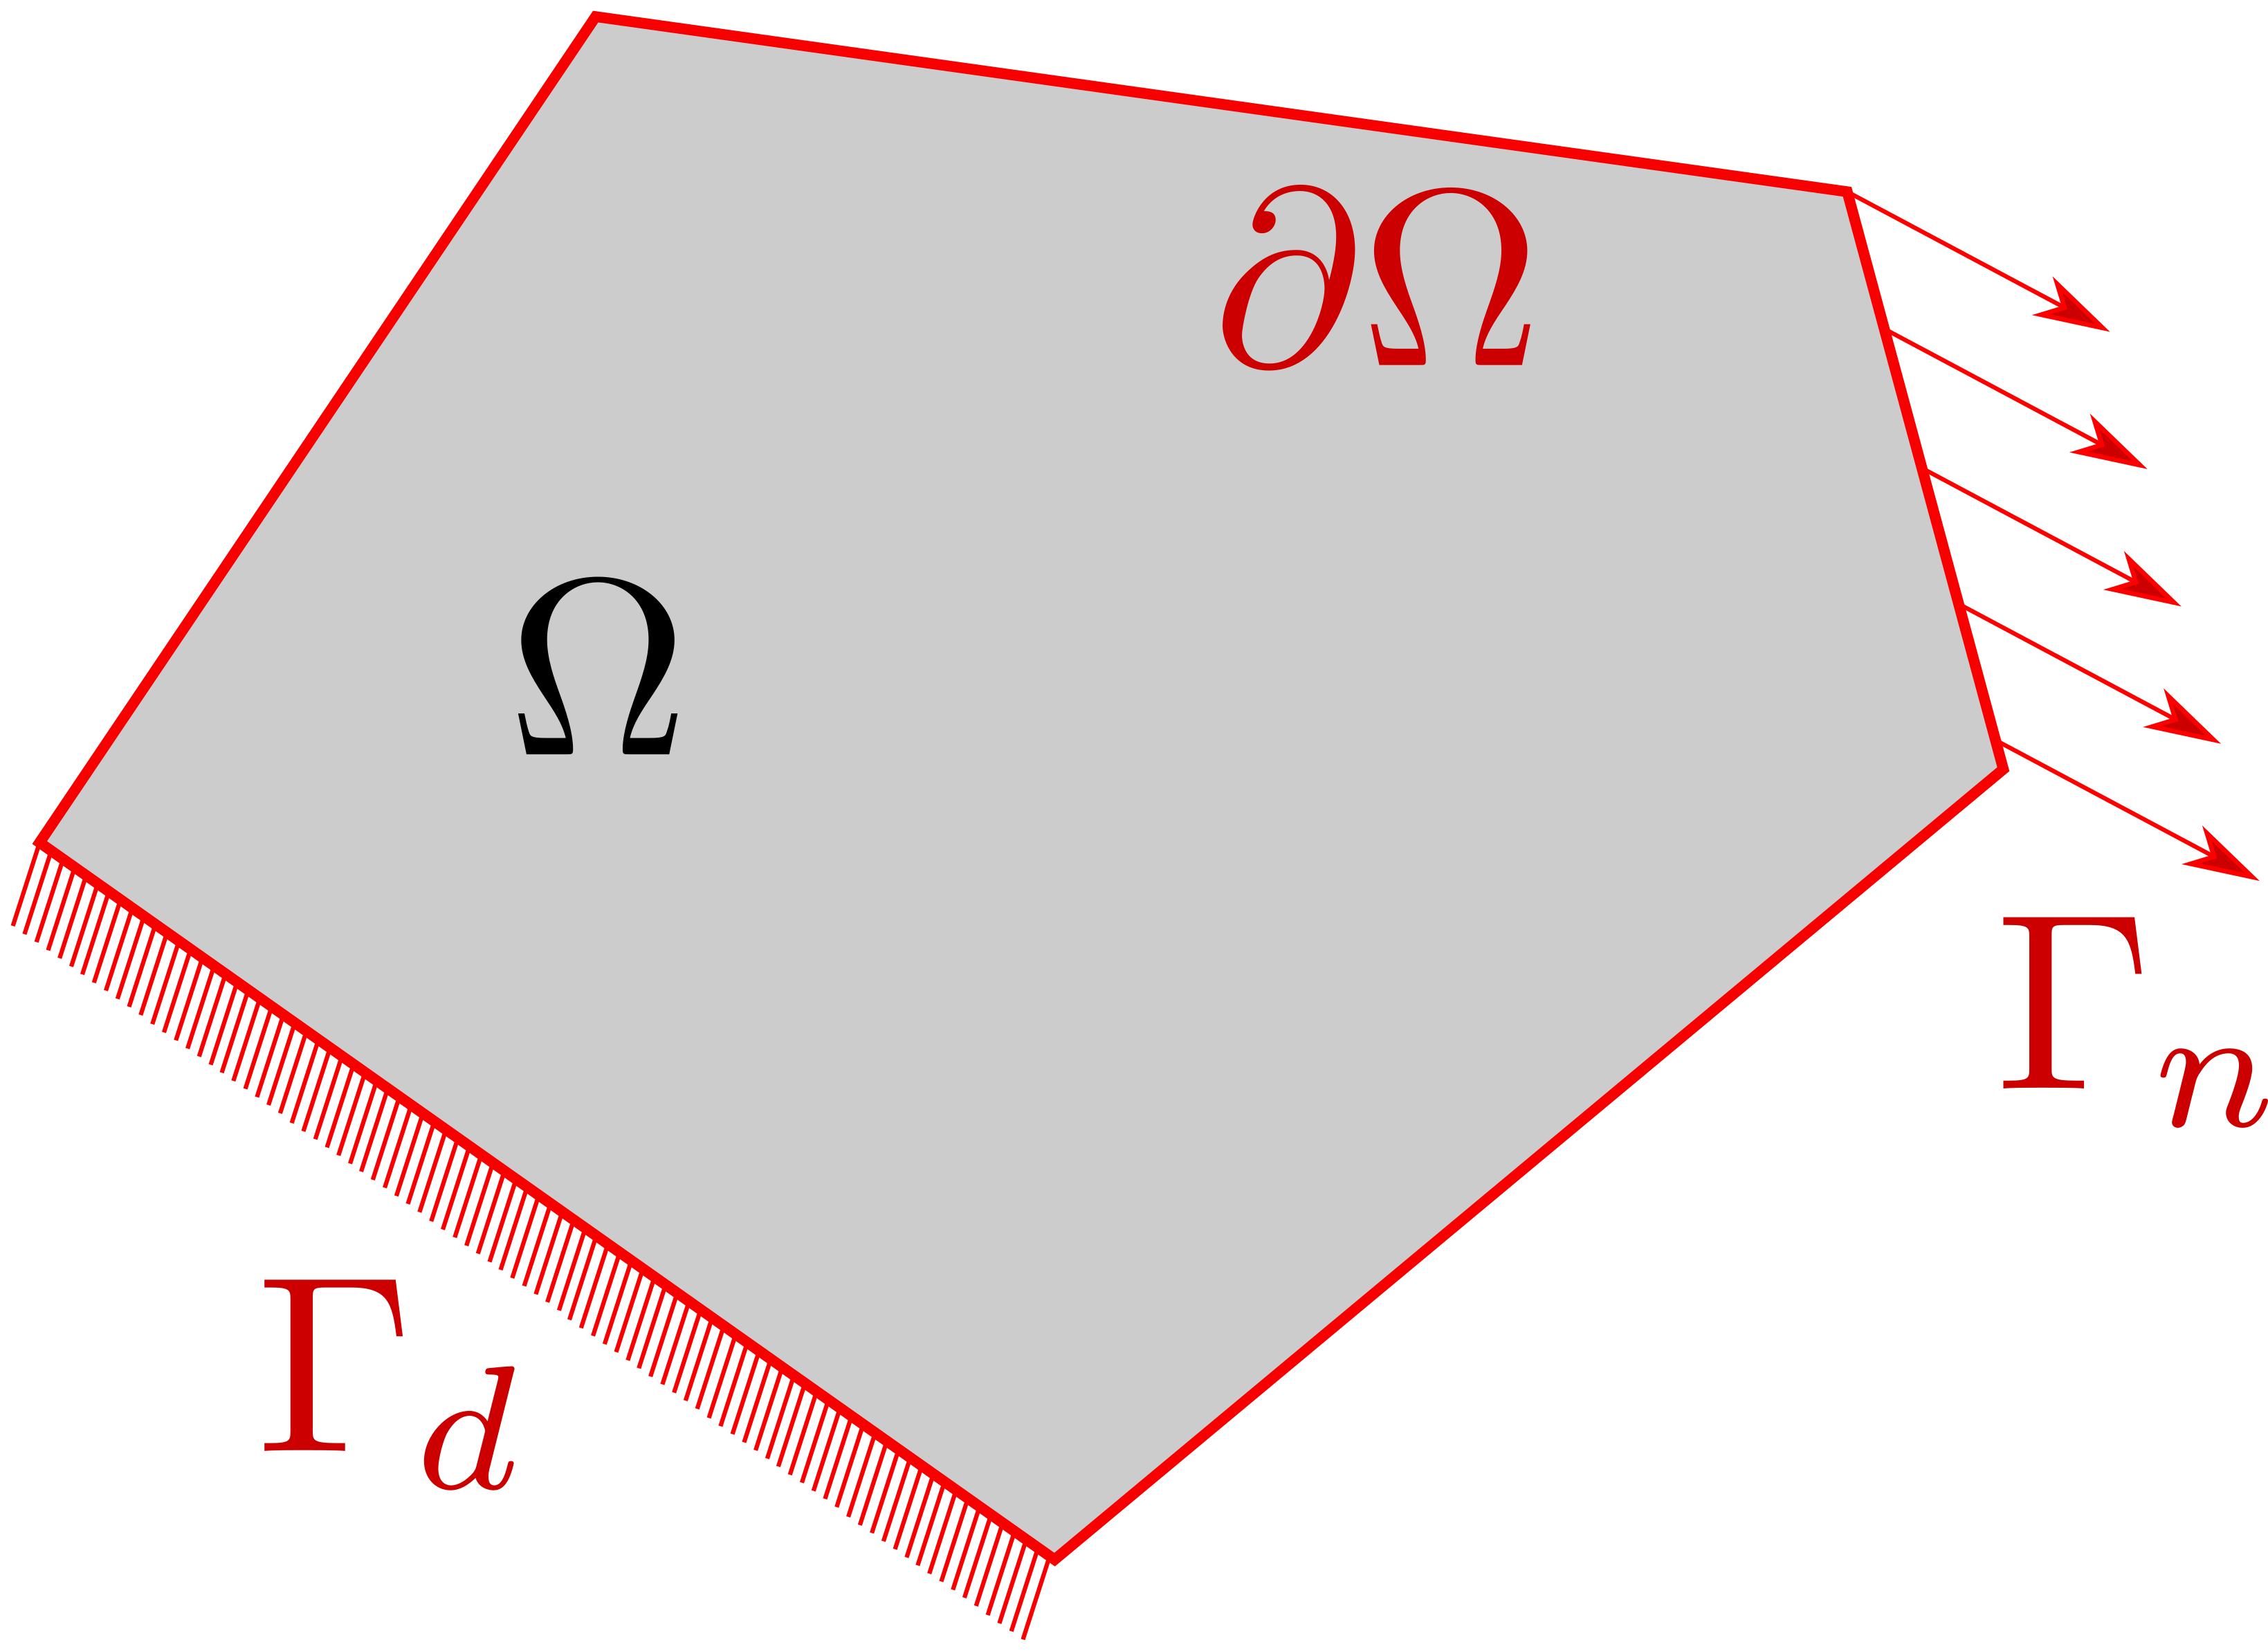
\includegraphics[width=\textwidth]{Figures/Continuum-solid}}
  \caption{Description of the boundary-value-problem in a
    continuum. Red lines represents the closure $\partial \varOmega$
    of the domain $\varOmega$ represented in gray.}
  \label{fig:Continuum-solid}
\end{figure}
%%%%%%%%%%%%%%%%%%%%%%%%%%%%%%%%%%%%%%%%%%%%%%%%%%%%%%%%%%%%%%%%%%%%%%%%%%
In this context the field $\vect{u}$ allows to describe the \textit{global state}
of the system. Now the variable $\phi =
(\tens{\varepsilon},\tens{\sigma})$ is defined as the set of \textit{local
  states} at any point of the continuum which can be derived from the
field $\vect{u}$ through the following set of governing equations and
restrictions that must be satisfied. First (i) the \textit{compatibility
  equation} that extracts from $\vect{u}$ the strain field is,
\begin{equation}
  \label{eq:Compatibility-equation}
  \tens{\varepsilon} = \GradS{\vect{u}},
\end{equation}
together with essential boundary conditions of Dirichlet type
$\varGamma_d$. An additional consideration over the strain field is
the assumption of inifinitesimal strain, therefore second order terms
in the spatial derivatives can be neglected. The corresponding
conjugate variable for the strain field if the stress field
$\tens{\sigma}$, which satisfies (ii) the \textit{conservation of
  momentum equation}
\begin{equation}
  \label{eq:Balance-momentum}
\rho \frac{D\vect{v}}{Dt} = \Div{\tens{\sigma}} + \rho \vect{b}
\end{equation}
together with the natural boundary conditions of the Neumann type
$\varGamma_n$. Next (iii) the constitutive equation as a linear
application from $\Re^n$ to  $\Re^n$, which relates the
strain tensor with the stress tensor,
\begin{equation}
  \label{eq:Constitutive-equation}
\tens{\sigma} = \tens{D} \colon \tens{\varepsilon}.
\end{equation}
The final restriction is (iv) the mass conservation, which can be obtained by
setting to zero the total derivative of the density field,
\begin{equation}
  \label{eq:Rho-material-derivative}
  \frac{D \rho}{D t} = \dot{\rho} + \rho \Div{\vect{v}} = 0.
\end{equation}

\subsection{Variational formulation}
\label{sec:variational-formulation}
To write the variational statement of the problem, let us define a
virtual displacement field such that
\begin{equation}
  \label{eq:Hilbert-space}
  \vect{u}^{\psi} \in \mathcal{H}^1_0(\Omega) = \{ \vect{u}^{\psi} \in
  \mathcal{H}^1 \mid \vect{u}^{\psi} = \vect{0}\ \text{on}\ \Gamma_d \}.
\end{equation}
And which satisfies that the Cauchy sequences are convergent in $\varOmega$
\begin{equation}
  \label{eq:cauchy-secuence}
  \Integral{3}{\vect{u}^{\psi}} < \infty\ \quad\text{and}\quad
  \Integral{3}{\tens{\varepsilon}^{\psi}} < \infty
\end{equation}
The principle of virtual work states that the equilibrium solution to
the boundary-value problem of elasticity is the function $\vect{u} \in
\mathcal{H}^1_0$ such that, for $\vect{u}^{\psi} \in
\mathcal{H}^1_0$, the following holds:
\begin{equation}
  \label{eq:BalanceMomentum_wf}
  \Integral{3}{\rho\ \left( \frac{d\vec{v}}{dt}\ - \vec{b} \right) \cdot \vec{u}^{\psi}} =
  \Integral{2}{\vec{t}\ \cdot \vec{u}^{\psi}} - \Integral{3}{\tens{\sigma} \colon
   \tens{\varepsilon}^{\psi}},
\end{equation}\\
therefore (\ref{eq:BalanceMomentum_wf}) together with
\eqref{eq:Constitutive-equation} and
\eqref{eq:Rho-material-derivative} represents the weak form
formulation of the problem.

\subsection{Galerkin procedure}
\label{sec:Galerkin-procedure}
In order to arrive to a finite set of equations, in contrast with the
FEM, in MPM a double discretization procedure is performed as we will
describe here below. First, the continuum domain
$\Omega$ is discretized with a finite sum of material points (in the
following particles), each one
represent a part of the discretized domain $\varOmega_p \subset
\varOmega$ with $p = 1,2\ldots ,N_p$ where $N_p$ is the number of
particles. The material point $\vec{x}_p$ is defined at the centroid
of each $\Omega_p$, figure~\ref{fig:MPM-discretization}.
Each material point is assigned with initial values of position,
velocity, mass, volume and stress denoted by $\vec{x}_p$,
$\vec{v}_p$, $m_p$,  $V_p$ and $\tens{\sigma}_p$, but also the
virtual displacement field $\vect{u}^{\psi}_{p}$. Therefore, employing
the definition of the material integral, where we recover the Riemann
integral definition as an addition of a finite set of points, and
their volumes are interpreted as quadrature weights. Consequently,
individual terms in \eqref{eq:BalanceMomentum_wf} are solved as follows. 
\begin{itemize}
\item Acceleration forces :
\begin{equation}
    \label{eq:particle_acceleration_forces}
    \Integral{3}{\rho\ \frac{d\vec{v}}{dt} \cdot \vect{u}^{\psi}} =
    \frac{d\vec{v}_{p}}{dt} \cdot \vect{u}^{\psi}_{p}\ m_p.
  \end{equation}\\
\item Internal forces :
  \begin{equation}
    \label{eq:particle_internal_forces}
    \Integral{3}{\tens{\sigma}\ \colon \tens{\varepsilon}^{\psi}} =
   \tens{\sigma}_{p}\ \colon \tens{\varepsilon}^{\psi}_p \ V_p.
  \end{equation}\\
\item Body forces :
\begin{equation}
  \label{eq:particle_body_forces}
  \Integral{3}{\rho\ \vec{b} \cdot \vect{u}^{\psi} } = 
  \vec{b}_{p} \cdot \vect{u}^{\psi}_p\ m_p.
\end{equation}\\
\item Loads :
\begin{equation}
  \begin{aligned}
    \label{eq:particle_load_forces}
    \Integral{2}{\vec{t}\ \vect{u}^{\psi}} = \Integral{2}{\rho\
      \vec{t}^s \cdot \vect{u}^{\psi}} = \vec{t}^s_{p} \cdot \vect{u}^{\psi}_{p}\ h^{-1}\ m_p ,
  \end{aligned} 
\end{equation}
\end{itemize}
where $h$ is the thickness of the continuum in a 2D case. Here is
where the second discretization procedure appears. A background mesh
composed by a finite set of grid points with coordinates $\vec{x}_I\
, I = 1,2\ldots ,N_n$, is generated. Where $N_n$ is the number of grid
nodes. This mesh is employed as a support to compute gradients and
divergences.
%%%%%%%%%%%%%%%%%%%%%%%%%%%%%%%%%%%%%%%%%%%%%%%%%%%%%%%%%%%%%%%%%%%%%%%%%%
\begin{figure}\sidecaption
  \centering
  \resizebox{0.5\hsize}{!}{
    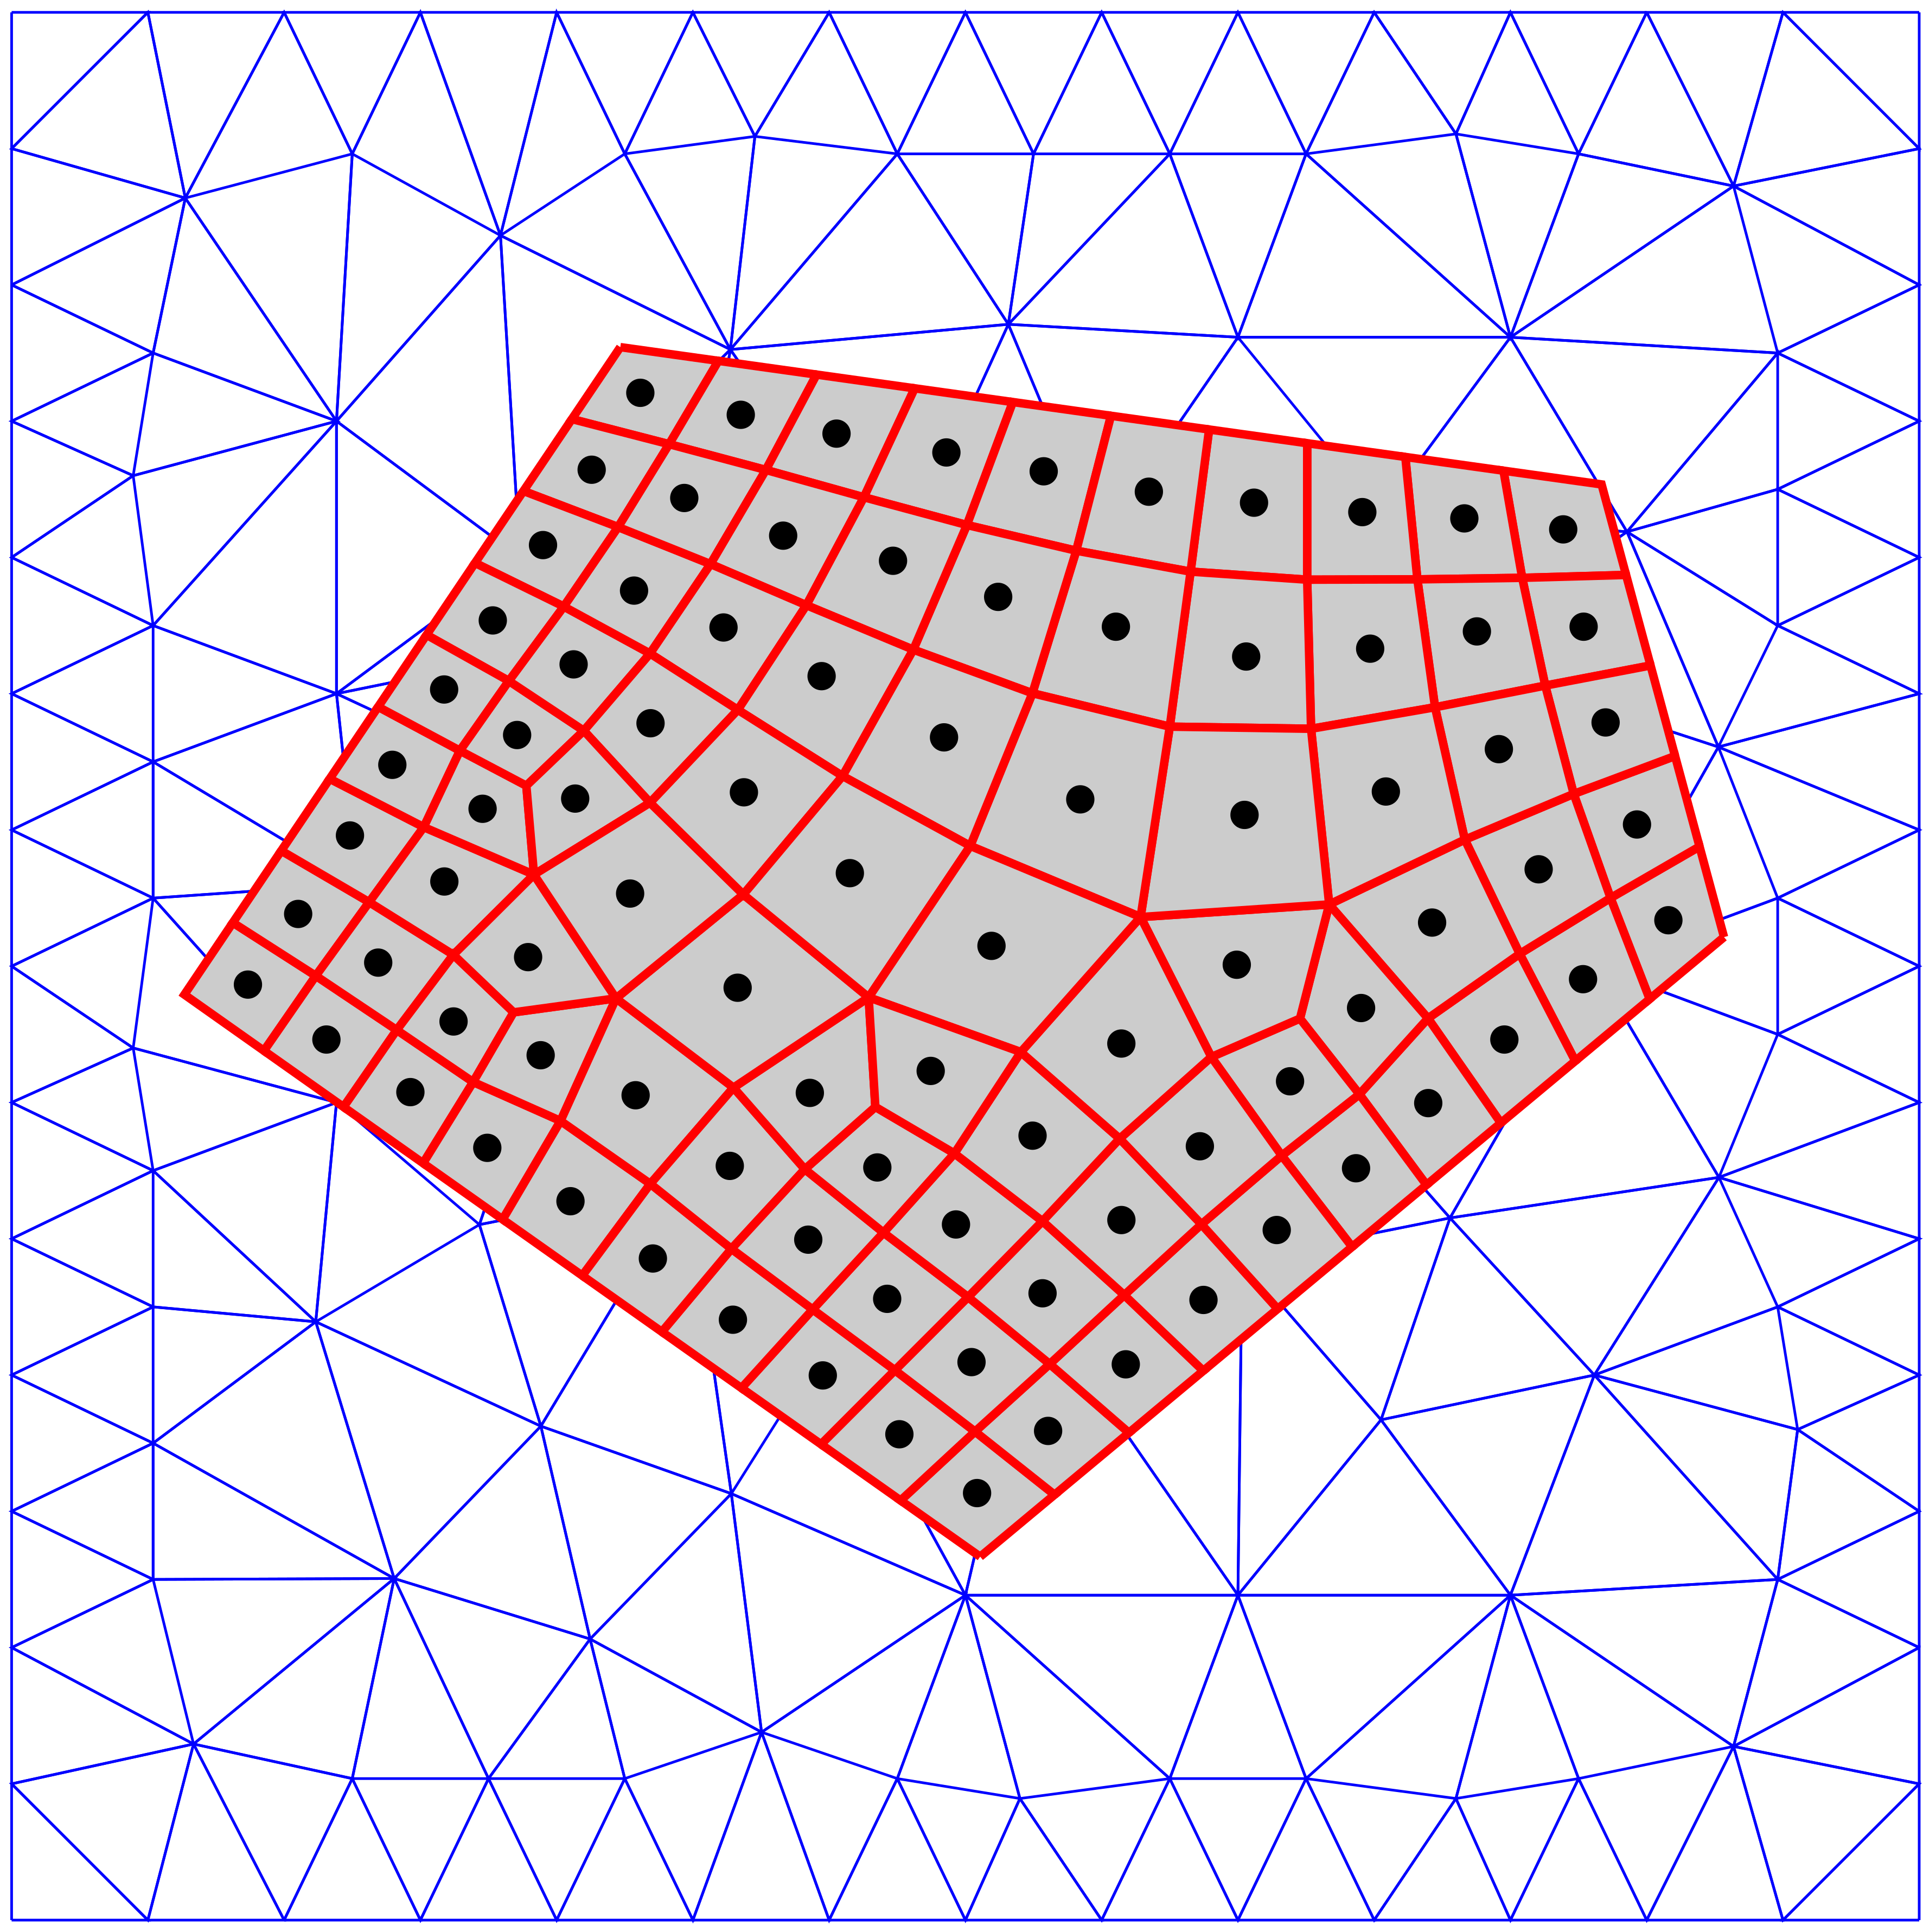
\includegraphics[width=\textwidth]{Figures/Mesh-particles-back}}
  \caption{Description of the spatial discretization for domain presented in the
    figure~\ref{fig:Continuum-solid}. Blue mesh represent the
    background computational support, and the grid mesh conforms the
    discretized continuum body.}
  \label{fig:MPM-discretization}
\end{figure}
%%%%%%%%%%%%%%%%%%%%%%%%%%%%%%%%%%%%%%%%%%%%%%%%%%%%%%%%%%%%%%%%%%%%%%%%%%
Introducing \eqref{eq:particle_acceleration_forces},
\eqref{eq:particle_internal_forces}, \eqref{eq:particle_body_forces}, 
and \eqref{eq:particle_load_forces} in \eqref{eq:BalanceMomentum_wf},
and approximating the displacement field of the particle
$p$ as $\vec{u}_{p} = N_{Ip} \vect{u}_I$, $\vec{u}^{\psi}_{p} = N_{Ip} \vect{u}_I^{\psi}$,
and its gradient as $\tens{\varepsilon}_p = (\vect{u}_I \otimes
\Grad{N_{Ip}})^s$, $\tens{\varepsilon}_p^{\psi}= (\vect{u}_I^{\psi} \otimes \Grad{N_{Ip}})^s$.
We reach to the nodal balance of forces of the continuum,
\begin{equation}
  \label{eq:particle_balance_forces3}
  \dot{\vec{p}}_{I}= \tens{m}_{IJ}\dot{\vec{v}}_{J} = \vec{f}_{I}^{int} + \vec{f}_{I}^{ext},
\end{equation}
where $\dot{\vec{p}}_{I}$ is the rate of momentum at grid node $I$, the nodal mass matrix $\tens{m}_{IJ}$ is,
\begin{equation}
  \label{eq:particle_nod_mass}
  \tens{m}_{IJ} = N_{Ip} m_p N_{Jp}.
\end{equation}
To improve the computational efficiency and stability, the nodal mass matrix
\eqref{eq:particle_nod_mass} can be substituted by the lumped mass
matrix $\tens{m}_{IJ}^{lumped}$.
Later, internal and external forces are computed as follows,
\begin{equation}
  \label{eq:nodal_internal_forces}
  \vec{f}_{I}^{int} = - \tens{\sigma}_{p} \cdot \Grad{N_{Ip}} \frac{m_p}{\rho_p}
\end{equation}
\begin{equation}
  \label{eq:nodal_external_forces}
  \vec{f}_{I}^{ext} = N_{Ip}\ \vec{b}_{p}\ m_p  + N_{Ip}\ \vec{t}^s_{p}\ m_p h^{-1} 
\end{equation}
where $\tens{\sigma}_{p} = \tens{\sigma}_{p}(\tens{\varepsilon}_{p})$
is the particle $p$ stress field, which can be integrated employing
the suitable constitutive model. The strain tensor is updated employing the rate of stress tensor $\dot{ \tens{\varepsilon}}_{p}$ used to update the
strain tensor is as follows \eqref{eq:IncrStrainPoint}.
\begin{equation}
  \label{eq:IncrStrainPoint}
  \dot{\tens{\varepsilon}_{p}} = \frac{\Delta
    \tens{\varepsilon}_{p}}{\Delta t} =
  \frac{1}{2} \left[\Grad{N_{Ip}}\ \otimes \vec{v}_{I} + \vec{v}_{I} \otimes
    \Grad{N_{Ip}}\ \right].
\end{equation}
Next, imposing $\frac{D \rho}{D t} = 0$, we ensures the mass
conservation and update the density field.
\begin{equation}
  \label{eq:MassConservation}
\dot{\rho} = - \rho\ \mathit{tra} \left( \dot{\tens{\varepsilon}} \right)
\end{equation}

Finally, to solve the equation \eqref{eq:particle_balance_forces3}, a second order
temporal integration scheme is required. Therefore, time is
discretized in to a finite set of time steps $k = 1\ldots ,Nt$, where $k$ is the current time step and $N_t$
is the total number of time steps. Once the nodal equilibrium equation it is solved, the values in the nodes are
interpolated back in to the particles and each particle it is advected
to the new position,
\begin{equation}
  \label{eq:Updated_Lagrangian}
  \dot{\vec{v}}_p = N_{Ip}\ \vec{a}_{I},\quad and\quad
  \dot{\vec{x}}_{p} = N_{Ip}\ \vec{v}_{I}  
\end{equation}
In MPM literature, this equations
(\ref{eq:particle_balance_forces3}) and (\ref{eq:Updated_Lagrangian}),
are solved with an explicit forward Euler algorithm. The time integration scheme of MPM has been described in detail by many researchers
\cite{Sulsky1994}, \cite{Bardenhagen2002}, \cite{thesis_Andersen_2009} and summarized
in figure~\ref{fig:MPM_algorithm}.
%%%%%%%%%%%%%%%%%%%%%%%%%%%%%%%%%%%%%%%%%%%%%%%%%%%%%%%%%%%%%%%%%%%%%%%%%%
\begin{figure}\sidecaption
  \centering
  \resizebox{0.5\hsize}{!}{
    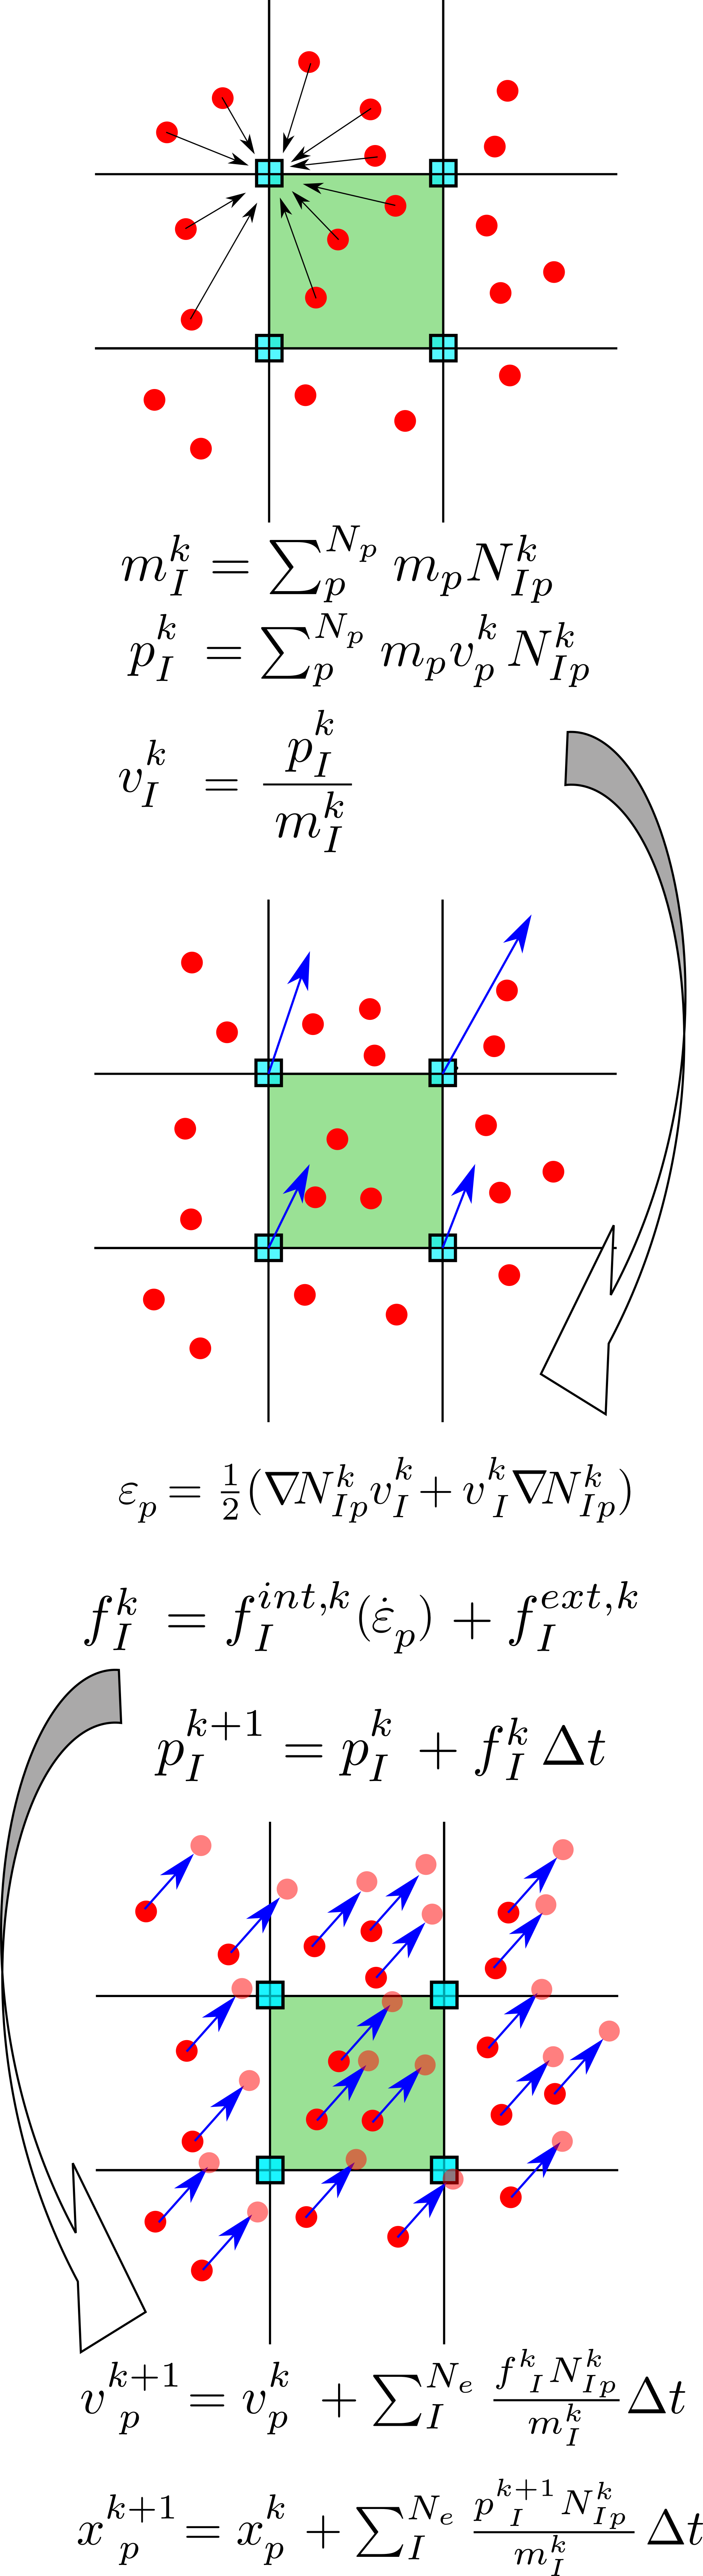
\includegraphics[width=\textwidth]{./Figures/MPM_scheme}
  }
  \caption{Description of the three steps in MPM standard algorithm.}
  \label{fig:MPM_algorithm}
\end{figure}
%%%%%%%%%%%%%%%%%%%%%%%%%%%%%%%%%%%%%%%%%%%%%%%%%%%%%%%%%%%%%%%%%%%%%%%%%%
Other authors have proposed many others time integration alternatives
like \cite{Guilkey2003}, \cite{Tran2019e}, \cite{Charlton2017}. In the
first publication on MPM \cite{Sulsky1994}, the nodal acceleration
was employed to update the particles as
\begin{equation}
  \label{eq:Sulsky-1994-UL-v}
  \vect{v}_p^{k+1} = \vect{v}_p^{k} + \Delta t\ N_{Ip}^{k}\ \vec{a}_{I}^{k}
\end{equation}
\begin{equation}
  \label{eq:Sulsky-1994-UL-x}
  \vect{x}_p^{k+1} = \vect{x}_p^{k} + \Delta t\ N_{Ip}^{k}\ \vec{v}_{I}^{k}.
\end{equation}
However, as Andersen (2009)\cite{thesis_Andersen_2009} point out, this algorithm has been shown to be numerically unstable due to that
$\vect{f}_I^{int,k}$ can be finite for an infinitesimal nodal mass
$\tens{m}$. This can lead to numerical issues when nodal acceleration
is obtained for evaluating \eqref{eq:Sulsky-1994-UL-x},\eqref{eq:Sulsky-1994-UL-v}. Hence, a
corrected version of this algorithm in shown in Zhang {\it et al.}
(2016)\cite{Zhang_book_2016}
\begin{equation}
  \label{eq:Zhang-2016-UL-x}
  \vect{x}_p^{k+1} = \vect{x}_p^{k} + \Delta t\ \frac{N_{Ip}^{k}\ \vec{p}_{I}^{k}}{\tens{m}_I}.  
\end{equation}
\begin{equation}
  \label{eq:Zhang-2016-UL-v}
  \vect{v}_p^{k+1} = \vect{v}_p^{k} + \Delta t\ \frac{N_{Ip}^{k}\ \vec{f}_{I}^{k}}{\tens{m}_I},
\end{equation}
Later Tran \& Solowski (2019)\cite{Tran2019e} presented a
generalized-$\alpha$ scheme for MPM inspired in the explicit time
integration algorithm proposed by Chung \& Hulbert
(1993)\cite{Geranlized_alpha_1993}, but with the particularity that
the acceleration is evaluated both in the beginning and the end of the
time step.
\begin{equation}
  \label{eq:Tran-2019-GA-v}
  \vect{v}_p^{k+1} = \vect{v}_p^{k} + \Delta t\  N_{Ip}^{k}\ \left[(1 - \gamma)\ \vect{a}_I^{k} +
    \gamma\ \vect{a}_I^{k+1} \right],\\
\end{equation}
\begin{equation}
\label{eq:Tran-2019-GA-x}
  \vect{x}_p^{k+1} = \vect{x}_p^{k} + N_{Ip}^{k} \left[ \Delta t\ \vec{v}_{I}^{k}+ \Delta t^2\left( (\frac{1}{2} - \beta)\
    \vec{a}_{I}^{k} + \beta\ \vec{a}_{I}^{k+1} \right) \right]
\end{equation}
\begin{equation}
  \label{eq:Tran-2019-GA-a}
  \vect{a}_p^{k+1} = N_{Ip}^{k}\ \vec{a}_{I}^{k+1}.
\end{equation}

This scheme has prof to damps out the higher frequency noises
\cite{Tran2019e}. But it can present the same numerical instabilities
as in \eqref{eq:Sulsky-1994-UL-x},\eqref{eq:Sulsky-1994-UL-v} when
nodal masses become infinitesimal, and requires extra storage for
nodal values of acceleration and previous steps.  

\section{Explicit predictor-corrector scheme for MPM.}
\label{sec:epc-algor-mpm}

In this section, a explicit predictor-corrector time integration
scheme is presented. It is based in the Newmark a-form 
$\gamma = 0.5$ and $\beta = 0$ which is the central difference
explicit. This method is devoted to solve a system of equations of the type
\begin{equation*}
  \Matrix{M}_{IJ}\ddot{\Vector{d}}_{J} + \Matrix{C}_{IJ}\dot{\Vector{d}}_{J} +
  \Matrix{K}_{IJ}\Vector{d}_{J} = \Vector{F}_{I}.
\end{equation*}
As MPM has a nodal stage, it is possible to apply this methods
successfully in MPM framework as was proved by
\cite{Tran2019e}. Taking the predictor definition from and calculating
nodal velocity, and updating particles position employing nodal values
of velocity and acceleration. The predictor-corrector algorithm has
been described in the classic literature \cite{Hughes2000}, and its
computational advantages and stability were widely proof by Liu
\cite{Xiaojian94}. The ``classic'' PCE algorithm starts with a
predicted value of the nodal velocity at the $(k+1)$th time step denoted by $\vec{\tilde{v}}_I^{k+1}$ given as,
\begin{equation}
  \label{eq:Predictor-velocity-I}
  \vec{\tilde{v}}_I^{k+1} = \vec{v}_I^k + (1 - \gamma)\ \Delta t\ \vec{a}_I^k
\end{equation}
In \eqref{eq:Predictor-velocity-I} arise a \textit{user-defined}
parameter $\gamma \geq 0$. This parameter influences both the predictor accuracy
and the stability of the algorithm. As point out Liu
\cite{Xiaojian94}, the truncation error of the predictor formula is
$O(\Delta t^3)$ when $\gamma = 0.5$, and is unconditionally stable if
$ 0 < \gamma \leq 0.25$.

To accommodate this step to MPM framework, it is necessary to get
the nodal values of the velocity and acceleration throughout a variational
recovery process where particles quantities are transferred to the
mesh nodes. This technique arise as a generalization of the super-convergent recovery
procedures described by Zienkiewicz \& Zhu \cite{ZZ1992_I} (\textit{ZZ})
in the context of FEM. In MPM Gauss quadrature is not employed as
integrals are computed following the Riemann integral definition,
where each component of the summation correspond to a particle of the
discretization. Also Bardenhagen \& Kober \cite{Bardenhagen2004}
proved that thorough this information-transference technique mass and momentum are conserved. So for a general particle variable $\Phi_p$ employing the
\textit{ZZ} technique is possible to get its nodal homologous $\Phi_I$  as,
\begin{equation}
  \label{eq:Variational-recovery}
   \Phi_I = \frac{m_p N_{Ip} \Phi_p}{m_I}
 \end{equation}
 Therefore, to get a analogous expression for
 \eqref{eq:Predictor-velocity-I} in the context of MPM, the
 procedure described in the equation \eqref{eq:Variational-recovery}
 is employed reaching to,
 \begin{equation}
   \label{eq:Predictor-velocity-II}
   \vec{\tilde{v}}_I^{k+1} = \underbrace{\frac{N_{Ip}^{k} m_p
       \vec{v}_p^k}{m_I}}_{\vec{v}_I^{k}} + (1 - \gamma)\ \Delta t\  \underbrace{\frac{N_{Ip}^{k} m_p \vec{a}_p^k}{m_I}}_{\vec{a}_I^{k}}
 \end{equation}
Nonetheless this way of computing the predictor stage can introduce
instabilities due to numerical cancellation likewise the original
Sulky algorithm. Thankfully this can be avoided easily by the
equivalent formulation \eqref{eq:Predictor-velocity-II}, 
\begin{equation}
  \label{eq:Predictor-velocity-II}
  \vec{\tilde{v}}_I^{k+1} = \frac{ N_{Ip}^{k} m_p (\vec{v}_p^k + (1 - \gamma)\ \Delta t\ \vec{a}_p^k)}{m_I}
\end{equation}
This way of computing the nodal predictor is both numerically stable
and minimize the computational effort. Once nodal velocity are
obtained, the essential boundary conditions are imposed. And in the
following, the ``classic'' MPM algorithm continues to reach to the
equilibrium equation \eqref{eq:particle_balance_forces3}. Here we
continue with the \textit{corrector} stage, due to the fact that we
already have nodal velocity, this step is computed in the same way as
in FEM,
\begin{equation}
  \label{eq:Corrector-velocity}
  \vec{v}_{I}^{k+1} = \vec{v}_{I}^{pred} + \gamma\ \Delta t\ \frac{\vec{f}_{I}^{k+1}}{\tens{m}_I^{k+1}}
\end{equation}
Finally updated particle kinetics are computed using nodal values as,
\begin{align}
  \label{eq:Update-lagrangian-pce}
        &\vec{a}_p^{k+1} = \vec{a}_p^n +
        \frac{N_{Ip}^k\vec{f}_{I}^{k}}{\tens{m}_I^k}\\
      &\vec{v}_p^{k+1} = \vec{v}_p^n + \Delta t\
        \frac{N_{Ip}^k\
        \vec{f}_{I}^{k}}{\tens{m}_I^k}\\
      &\vec{x}_p^{k+1} = \vec{x}_p^n + \Delta t\
         N_{Ip}^k\ \vec{v}_{I}^{k} +
        \frac{1}{2}\Delta t^2\ \frac{N_{Ip}^k\
        \vec{f}_{I}^{k}}{\tens{m}_I^k} 
\end{align}
Notice that particle displacement is computed using the corrected
nodal velocities and the accelerations computed with the velocities
of the predictor. However, particles velocities and accelerations
are computed using the corrected velocities. Therefore here we share similarities
with the \textit{leapfrog integration} which updates the position at
full time step, but updates the velocity at half time steps. Notice
also that with this approach the calculation of nodal momentum values
are not required. Due to its simplicity allows be implemented with minor modifications
over a standard forward Euler. It is summarized in shape of
pseudo-algorithm.

\begin{algorithm}
  \floatname{algorithm}{Algorithm}
  \renewcommand{\thealgorithm}{}
  \caption{Explicit Predictor-Corrector scheme}
  \begin{algorithmic}[1]
    %%%%%%%%%%%%%%%%%%%%%%%%%%%%%%%%%%%%%%%%%%%%%%%%%%%%%%%%%%%%%%%%%%%%%%%%%%%%%%%%%%%%%% º
    \STATE \textbf{Update mass matrix}:
    \begin{equation*}
      \tens{m}_{I} = N_{Ip}^{k}\ m_p,
    \end{equation*}
    %%%%%%%%%%%%%%%%%%%%%%%%%%%%%%%%%%%%%%%%%%%%%%%%%%%%%%%%%%%%%%%%%%%%%%%%%%%%%%%%%%%%%% 
    \STATE \textbf{Explicit Newmark Predictor}:\\
    \begin{equation*}
      \vec{v}_I^{pred} = \frac{ N_{Ip}^{k} m_p (\vec{v}_p^k + (1 - \gamma)\ \Delta t\ \vec{a}_p^k)}{m_I}
    \end{equation*}
    %%%%%%%%%%%%%%%%%%%%%%%%%%%%%%%%%%%%%%%%%%%%%%%%%%%%%%%%%%%%%%%%%%%%%%%%%%%%%%%%%%%%%% 
    \STATE \textbf{Impose essential boundary conditions}:\\
    At the fixed boundary, set $\vec{v}_{I}^{pred} = 0$. 
    %%%%%%%%%%%%%%%%%%%%%%%%%%%%%%%%%%%%%%%%%%%%%%%%%%%%%%%%%%%%%%%%%%%%%%%%%%%%%%%%%%%%%% 
    % \STATE \textbf{Discard the previous nodal values}.
    %%%%%%%%%%%%%%%%%%%%%%%%%%%%%%%%%%%%%%%%%%%%%%%%%%%%%%%%%%%%%%%%%%%%%%%%%%%%%%%%%%%%%% 
    \STATE \textbf{Deformation tensor increment calculation}.
    \begin{align*}
      &\dot{\tens{\varepsilon}_{p}}^{k+1} = \left[ \vec{v}_{I}^{pred} \otimes
        \Grad{N_{Ip}^{k+1}} \right]^s \\
      &\Delta \tens{\varepsilon}_{p}^{k+1} = \Delta t\ \dot{\tens{\varepsilon}_{p}}^{k+1}
    \end{align*}
    %%%%%%%%%%%%%%%%%%%%%%%%%%%%%%%%%%%%%%%%%%%%%%%%%%%%%%%%%%%%%%%%%%%%%%%%%%%%%%%%%%%%%% 
    \STATE \textbf{Update the density field}:
    \begin{equation*}
      \rho_p^{k+1} = \frac{\rho_p^k}{1 + \mathit{tra}\left[\Delta\tens{\varepsilon}_{p}^{k+1}\right]}.
    \end{equation*}
    %%%%%%%%%%%%%%%%%%%%%%%%%%%%%%%%%%%%%%%%%%%%%%%%%%%%%%%%%%%%%%%%%%%%%%%%%%%%%%%%%%%%%% 
    \STATE \textbf{Balance of forces calculation}:\\
    Calculate the total grid nodal force $\vec{f}_{I}^{k+1} =
    \vec{f}_{I}^{int,k+1} + \vec{f}_{I}^{ext,k+1}$ evaluating
    \eqref{eq:nodal_internal_forces} and
    \eqref{eq:nodal_external_forces} in the time step $k+1$.
    In the grid node $I$ is fixed in one of the spatial dimensions, set it to
    zero to make the grid nodal acceleration zero in that direction.\\
    %%%%%%%%%%%%%%%%%%%%%%%%%%%%%%%%%%%%%%%%%%%%%%%%%%%%%%%%%%%%%%%%%%%%%%%%%%%%%%%%%%%%%% 
    \STATE \textbf{Explicit Newmark Corrector}:
    \begin{equation*}
      \vec{v}_{I}^{k+1} = \vec{v}_{I}^{pred} + \gamma\ \Delta t\ \frac{\vec{f}_{I}^{k+1}}{\tens{m}_I^{k+1}}  
    \end{equation*}
    %%%%%%%%%%%%%%%%%%%%%%%%%%%%%%%%%%%%%%%%%%%%%%%%%%%%%%%%%%%%%%%%%%%%%%%%%%%%%%%%%%%%%%
    \STATE \textbf{Update particles lagrangian quantities}:
    \begin{align*}
      &\vec{a}_p^{k+1} = \vec{a}_p^n +
        \frac{N_{Ip}^k\vec{f}_{I}^{k}}{\tens{m}_I^k}\\
      &\vec{v}_p^{k+1} = \vec{v}_p^n + \Delta t\
        \frac{N_{Ip}^k\
        \vec{f}_{I}^{k}}{\tens{m}_I^k}\\
      &\vec{x}_p^{k+1} = \vec{x}_p^n + \Delta t\
         N_{Ip}^k\ \vec{v}_{I}^{k} +
        \frac{1}{2}\Delta t^2\ \frac{N_{Ip}^k\
        \vec{f}_{I}^{k}}{\tens{m}_I^k}
    \end{align*}
    %%%%%%%%%%%%%%%%%%%%%%%%%%%%%%%%%%%%%%%%%%%%%%%%%%%%%%%%%%%%%%%%%%%%%%%%%%%%%%%%%%%%%% 
    \STATE \textbf{Reset nodal values}
  \end{algorithmic}
\end{algorithm} 


\section{Local max-ent approximants}
\label{sec:local-max-ent}
The popularity of MPM has increase notoriously during
the recent years due to its ability to deal with large strain problems
without mesh distorsion issues inherent to mesh based methods like
FEM, see Zdzislaw \cite{Wieckowski2004}. However, in the simulations
made with the original MPM, there are numerical noises when particles
crossing the cell boundaries. Local maximum-entropy (or
local \textit{max-ent}) shape function first introduced by Arroyo \&
Ortiz (2006)\cite{Arroyo2006} has been recently tested under MPM framework
by Wobbes {\it et al.} (2020)\cite{Wobbes2020} where they prof that
simulations performed with the \textit{max-ent} basis functions show
considerably more accurate stress approximations for MPM. Although, in
\cite{Wobbes2020} authors does not deep in how the regularization
parameter $\beta$ affects to the accuracy and stability of the solution.

The basic idea of the shape functions based on such
an estimate is to interpret the shape function $N_I(\vec{x})$ as the
probability of $\vec{x}$ to obtain the value $\vec{x}_I$,  $I=1,
\dots, n$. Here $n$ is the number of nodes in the domain.
This approximation scheme represents a optimal compromise, in the sense of
Pareto, between the \textit{unbiased statistical inference} based on
the nodal data which leads to the principle of \textit{maximum-entropy}
stated by Jaynes \cite{Jaynes1957}, and the definition of local shape
functions of \textit{least width} the least biased shape functions.

Taking the definition of entropy as a measure of how uncertainty a
random variable is averaged on all its possible outcomes. And adopting
the Shannon's entropy as the starting point:
\begin{equation}
  \label{eq:Shannon-entropy}
  H(p_1(\vec{x}),\ldots,p_n(\vec{x})) = -\sum^{N_n}_{I=1}{p_I(\vec{x})\log p_I }
\end{equation}
where $p_I(\vec{x})$ is the probability, equivalent to the mentioned
shape function $N_I(\vec{x})$,  satisfying both the zeroth and
first-order consistency. The least-biased approximation scheme is
given by
\begin{align*}
  \label{eq:least-biased-approximation-scheme}
  \text{(LME)} \hspace{0.15cm} &\text{Maximize} \hspace{0.15cm} H(p) =
  -\sum_{I}^{N_n}{p_I(\vec{x})\log p_I }\\
  &\text{subject to}\
  \begin{cases}
    p_I \ge 0, \hspace{0.15cm} \text{I=1, ..., n} \\[1em]   
    \sum\limits_{I=1}^{N_n}{p_I} = 1 \\[1em]   
    \sum\limits_{I=1}^{N_n}{p_I \vec{x}_I} = \vec{x} \\
  \end{cases}
\end{align*}
The local max-ent approximation schemes (LME) as a Pareto set,
defined by \cite{Arroyo2006} is as follows
\begin{align*}
  \label{eq:LME-scheme-pareto-set}
  \text{(LME)}_{\beta} \hspace{0.15cm} &\text{For fixed} \hspace{0.15cm}
  \vec{x} \hspace{0.15cm} \text{minimise} \hspace{0.15cm} f_{\beta}(\vec{x}, p) = \beta H(\vec{x},p) - H(p) \\
  &\text{subject to}\
  \begin{cases}
    p_I \ge 0, \hspace{0.15cm} \text{I=1, ..., n} \\[1em]   
    \sum\limits_{I=1}^{N_n}{p_I} = 1 \\[1em]   
    \sum\limits_{I=1}^{N_n}{p_I \vec{x}_I} = \vec{x} \\
  \end{cases}
\end{align*}
for $\beta \in (0,\infty)$ is Pareto optimal. The unique solution of
the local max-ent problem (LME)$_\beta$ is: 
\begin{equation}
  \label{eq:LME-p}
p(\vec{x})=\frac{\exp\left[ -\beta \; |\vec{x}-\vec{x}_I|^2 +
    \vec{\lambda} \cdot (\vec{x}-\vec{x}_I) \right] } {Z(\vec{x},\vec{\lambda}^*(\vec{x}))}
\end{equation}
where
\begin{equation}
  \label{eq:LME-Z}
Z(\vec{x}, {\vec{\lambda}}) = \sum_{I=1}^{N_n}{ \exp \left[ -\beta \; |\vec{x}-\vec{x}_I|^2 + \vec{\lambda} \cdot (\vec{x}-\vec{x}_I)  \right]}
\end{equation}
being $\vec{\lambda}^*(\vec{x})$ the unique minimiser  for $\log
Z(\vec{x}, \vec{\lambda})$. In order to obtain the first derivatives of the shape function, it is also necessary to compute~$\nabla p^*_I$ 
\begin{equation}
  \label{eq:LME-grad-p}
\nabla p^*_I=p^*_I  \, \left(\nabla f^*_I-\sum_J^{N_n} p^*_J \, \nabla f^*_J\right)
\end{equation}
where
\begin{equation}
  \label{eq:LME-f}
f^*_I(\vec{x},  \vec{\lambda},\beta)=-\beta \, |\vec{x}-\vec{x}_I|^2 + \vec{\lambda}   \,  (\vec{x}-\vec{x}_I)
\end{equation}
Employing the chain rule, rearranging and considering $\beta$ as a constant, Arroyo and Ortiz~\cite{Arroyo2006} obtained the following expression:
\begin{eqnarray}
\nabla p^*_I &=& -p^*_I \,  (\tens{J}^*)^{-1} \,  (\vec{x} - \vec{x}_I) \label{eq26} 
\end{eqnarray}
%&&\mbox{
where \tens{J} is the Hessian matrix, defined by:
%} \nonumber \\&& \nonumber \\
\begin{eqnarray}
\tens{J}(\vec{x},  \vec{\lambda},\beta) &=& \frac{\partial \vec{r}}{\partial  \vec{\lambda}} \label{eq27} \\ 
%&& \nonumber \\
\vec{r}(\vec{x},\vec{\lambda},\beta) &\equiv& \partial_{\vec{\lambda}}{\log{ Z( \vec{x},\vec{\lambda}})} 
%\nonumber \\ &=&
  =\sum_I^{N_n} p_I(\vec{x},\vec{\lambda},\beta) \, (\vec{x} - \vec{x}_I) \label{eq28} 
\end{eqnarray}
Note that, the objective of the above procedure is to find the
$\vec{\lambda}$ which minimises  $\log Z(\vec{x}, \vec{\lambda})$. The
traditional way to obtain such a minimiser  is using Eq.~(\ref{eq27})
to calculate small increments of $\partial\vec{\lambda}$ in a
Newton-Raphson approach. Similar to alternative non-polynomial meshfree basis functions, the
LME approximation scheme requires more than $d+1$ nodes to determine
the values of the shape functions as well as their derivatives at any
point in the convex hull of the nodal set, where $d$ is the dimension
of the problem. The support size of LME shape functions may be
controlled by adjusting a dimensionless parameter, $\gamma=\beta h^2$
\cite{Arroyo2006} (e.g. two dimensional example shown in figure~\ref{fig:LME_MPM}).
 Since  $p_I$  is defined in the entire domain, in practice, the
function $\exp(-\beta \vec{r} )$ truncated  by  a given tolerance,
10$^{-6}$, for example,  would ensure a reasonable range of
neighbours, see \cite{Arroyo2006} for details. This tolerance defines
the limit values of the influence radius and is used thereafter to
find the neighbour nodes of a given integration point. Regarding this
aspect, an crucial consideration for the implementation of the LME
shape functions in MPM is exposed. To avoid the transference of
particle information to those nodes fare apart from the particle
domain $\Omega_p$, a especial treatment of the neighbour nodes for
those particles close to the boundary is required. It consists in
select only those nodes which position $\vect{x}_I$ lies inside of the
domain $\Omega$. This can be performed by employing the nodal
connectivity of the background mesh. And activating for computing only
those nodes whose element has a particle inside of it as we can see in
figure~\ref{fig:Particle-discretization}. 
%%%%%%%%%%%%%%%%%%%%%%%%%%%%%%%%%%%%%%%%%%%%%%%%%%%%%%%%%%%%%%%%%%%%%%%%%%
\begin{figure}\sidecaption
  \centering
  \resizebox{0.5\hsize}{!}{
    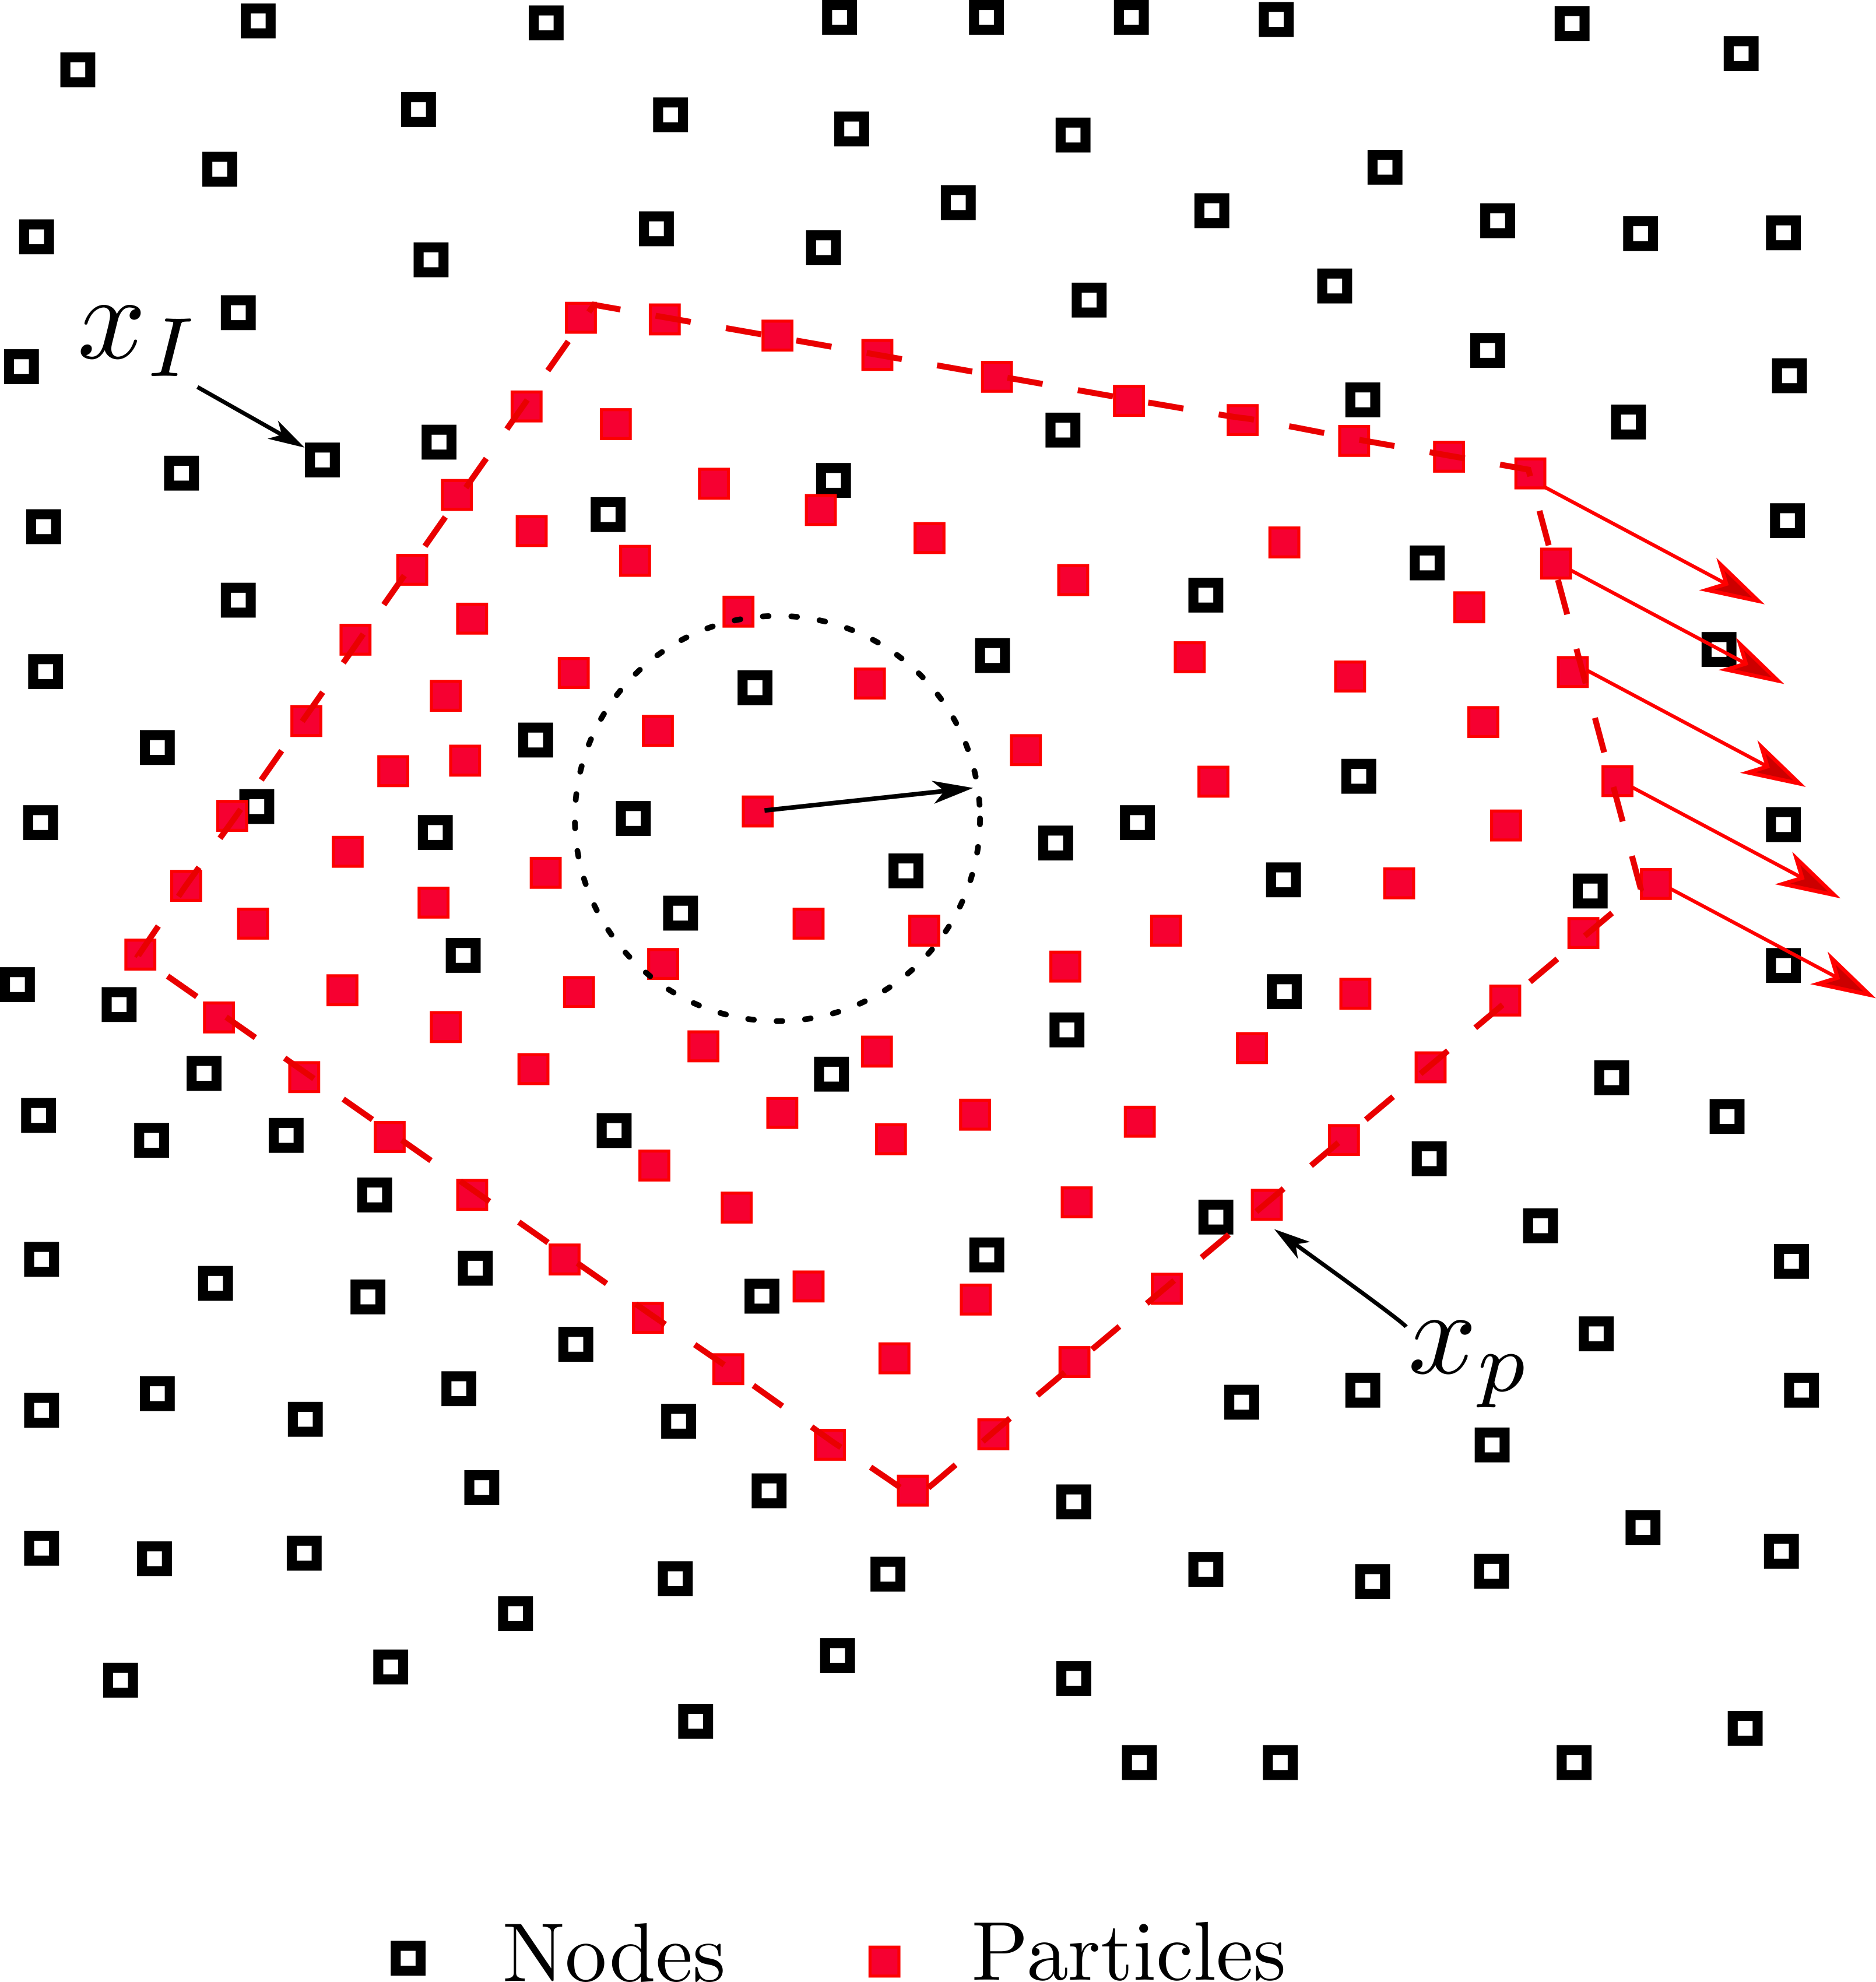
\includegraphics[width=\textwidth]{./Figures/Particle-discretization}
  }
  \caption{This tolerance defines the limit values of the influence
    radius and is used thereafter to find the neighbour nodes of a
    given integration point. The picture also shows the neighbourhood
    criterion to select those node inside of $\Omega$.} 
  \label{fig:Particle-discretization}
\end{figure}
%%%%%%%%%%%%%%%%%%%%%%%%%%%%%%%%%%%%%%%%%%%%%%%%%%%%%%%%%%%%%%%%%%%%%%%%%%
Due to the FE-compatibility, the LME shape function is degenerated to
linear finite element shape function if $d+1$ neighbouring nodes are
chosen as the support. Furthermore, with a conveniently adopted
\textit{regularization} parameter it is possible to get a GIMP-like
shape function. A proof of this statements is observed in figure~\ref{fig:LME_MPM}.  
%%%%%%%%%%%%%%%%%%%%%%%%%%%%%%%%%%%%%%%%%%%%%%%%%%%%%%%%%%%%%%%%%%%%%%%%%%
\begin{figure*}
  \centering
  \subfigure[Q4]{
    \begin{tabular}{c}
      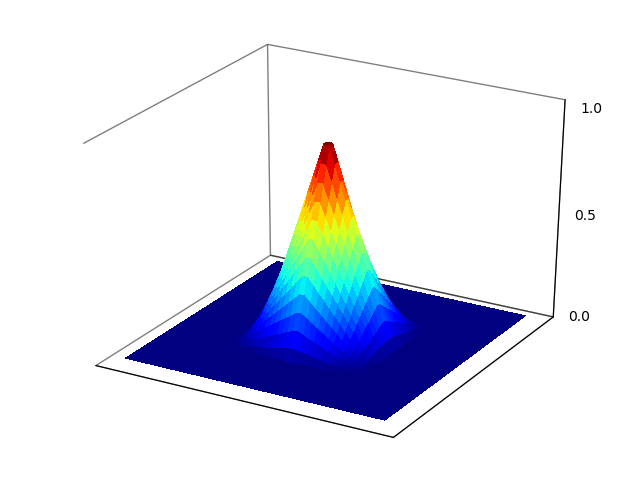
\includegraphics[width=0.14\textwidth]{Figures/MPM_Shape_Fun}\\
      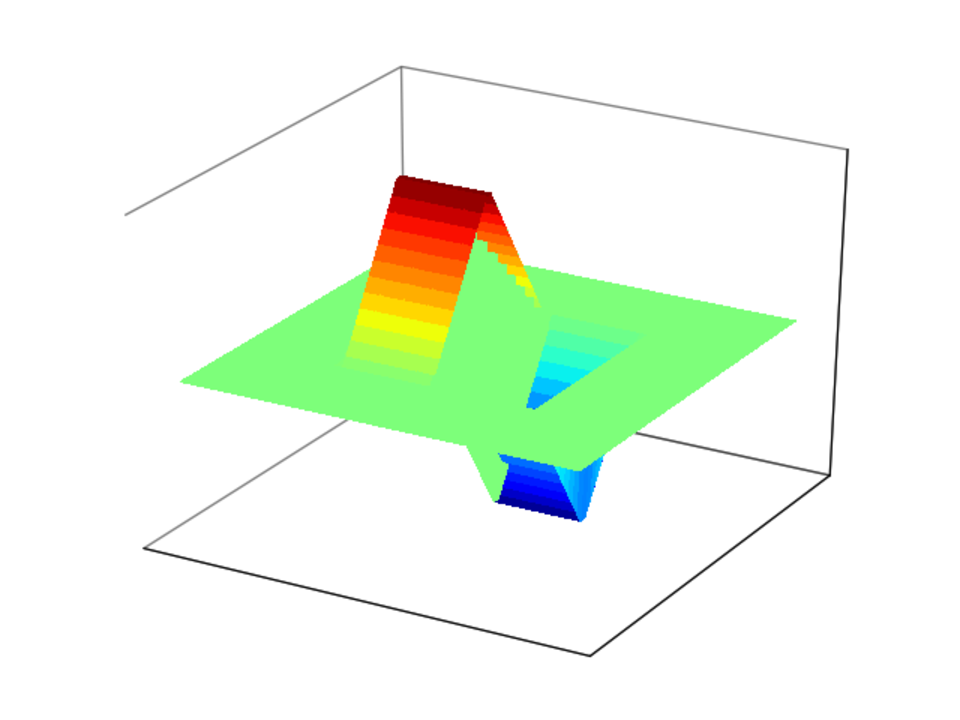
\includegraphics[width=0.14\textwidth]{Figures/MPM_Shape_Fun_dx}\\
      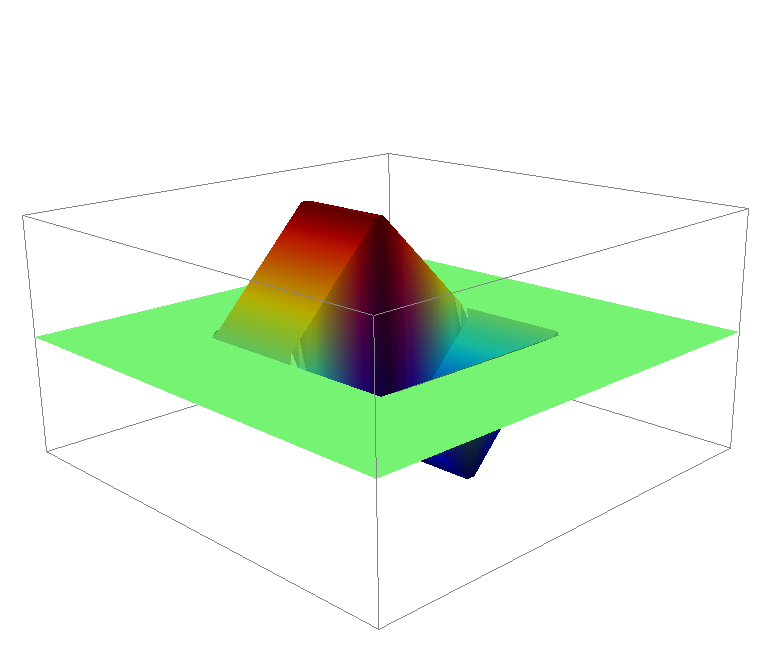
\includegraphics[width=0.14\textwidth]{Figures/MPM_Shape_Fun_dy}
    \end{tabular}  
  }
  \subfigure[$\text{LME}_{17}$]{
    \begin{tabular}{c}
      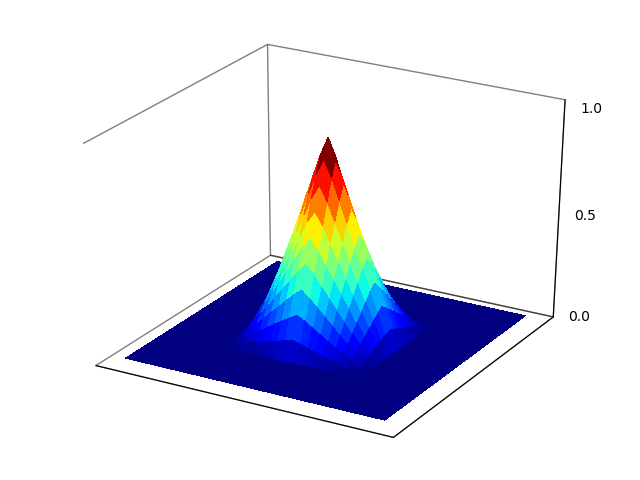
\includegraphics[width=0.14\textwidth]{Figures/LME_17_3_Shape_Fun}\\
      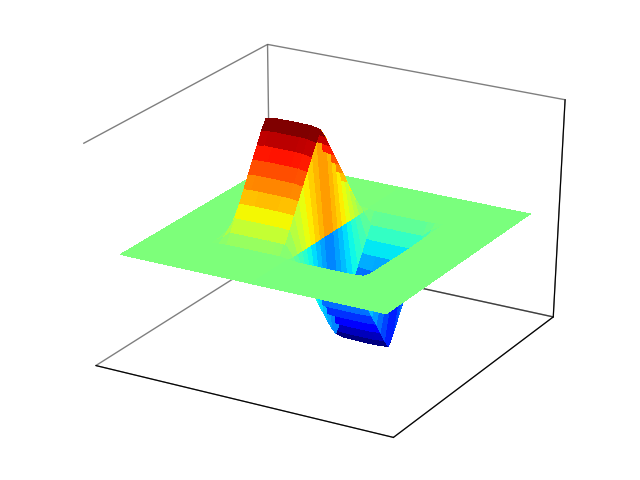
\includegraphics[width=0.14\textwidth]{Figures/LME_17_3_Shape_Fun_dx}\\
      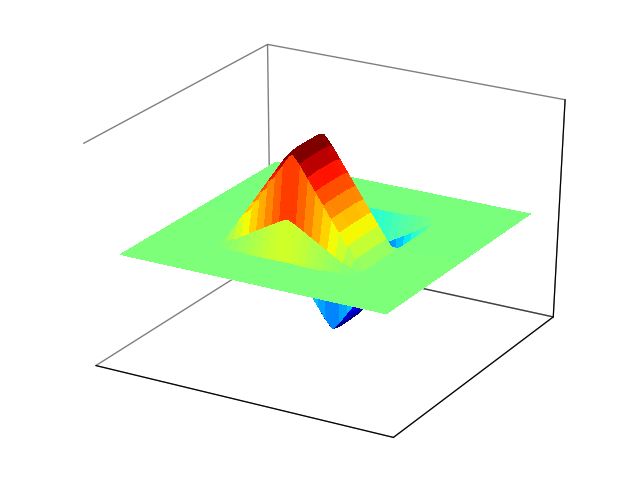
\includegraphics[width=0.14\textwidth]{Figures/LME_17_3_Shape_Fun_dy}
    \end{tabular}
  }
  \subfigure[uGIMP]{
    \begin{tabular}{c}
      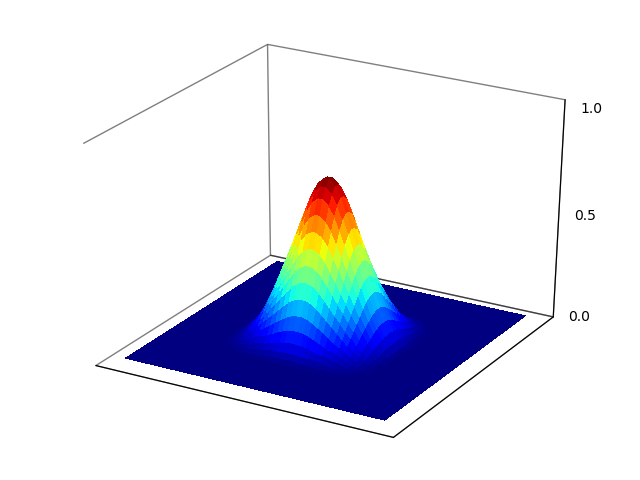
\includegraphics[width=0.14\textwidth]{Figures/GIMP_Shape_Fun}\\
      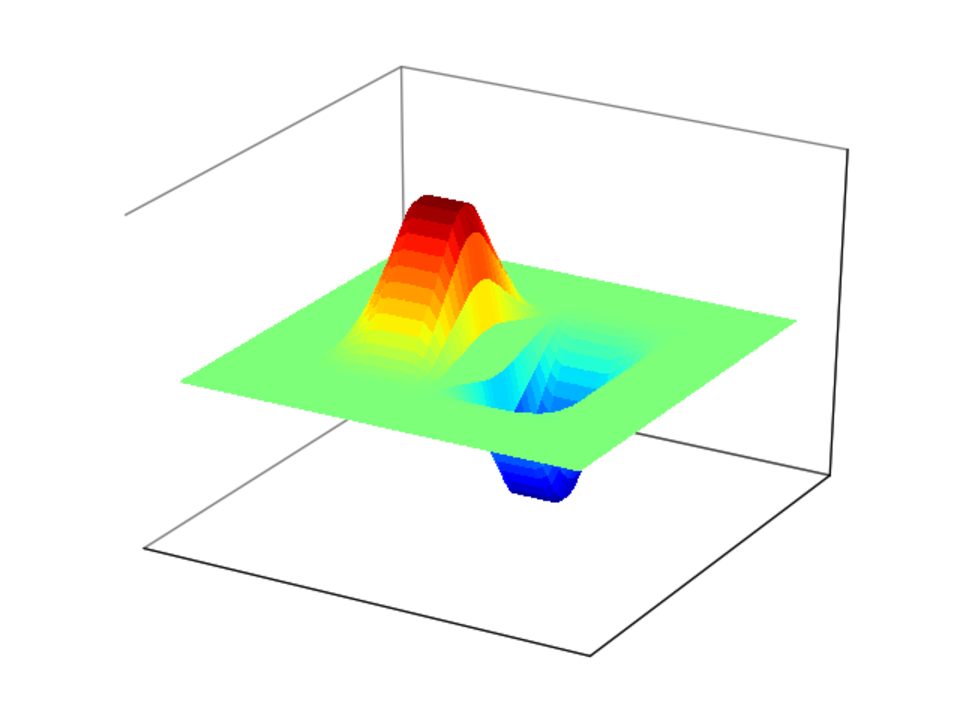
\includegraphics[width=0.14\textwidth]{Figures/GIMP_Shape_Fun_dx}\\
      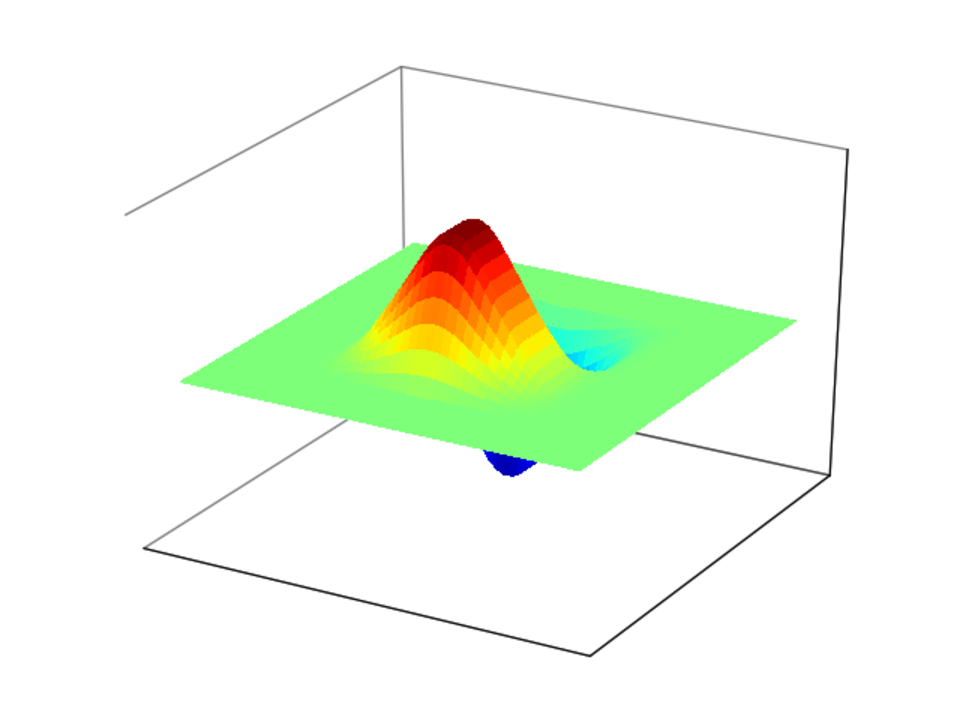
\includegraphics[width=0.14\textwidth]{Figures/GIMP_Shape_Fun_dy}
    \end{tabular}
  }
  \subfigure[$\text{LME}_{10}$]{
    \begin{tabular}{c}
      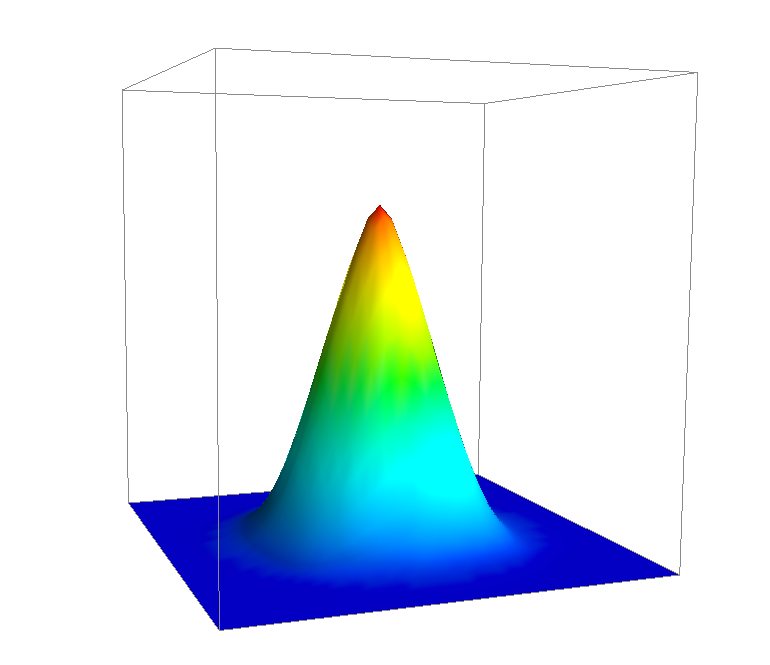
\includegraphics[width=0.14\textwidth]{Figures/LME_10_0_Shape_Fun}\\
      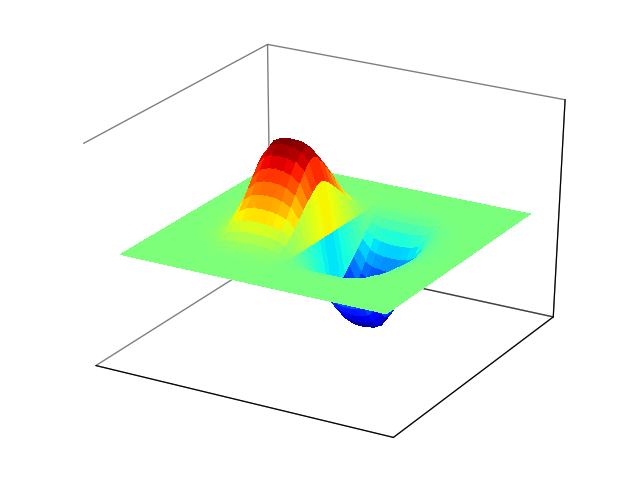
\includegraphics[width=0.14\textwidth]{Figures/LME_10_0_Shape_Fun_dx}\\
      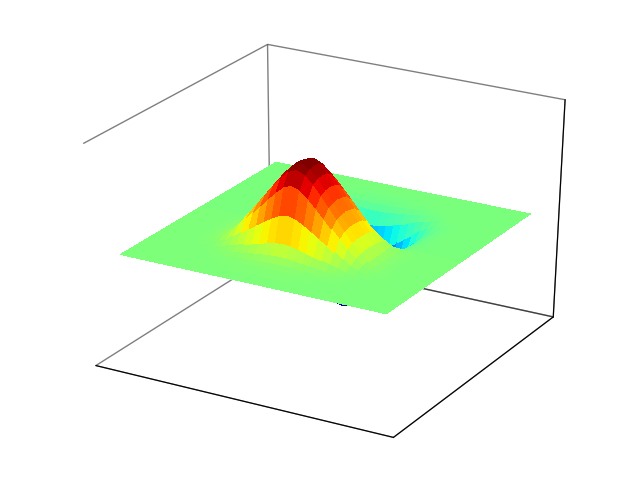
\includegraphics[width=0.14\textwidth]{Figures/LME_10_0_Shape_Fun_dy}    
    \end{tabular}
  }
  \subfigure[$\text{LME}_{5}$]{
    \begin{tabular}{c}
      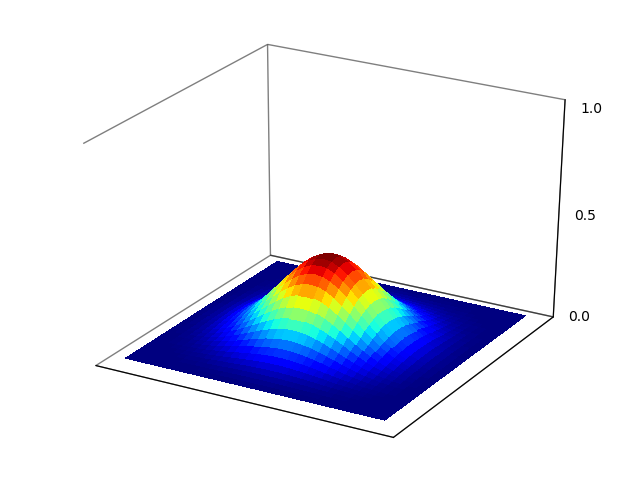
\includegraphics[width=0.14\textwidth]{Figures/LME_5_0_Shape_Fun}\\
      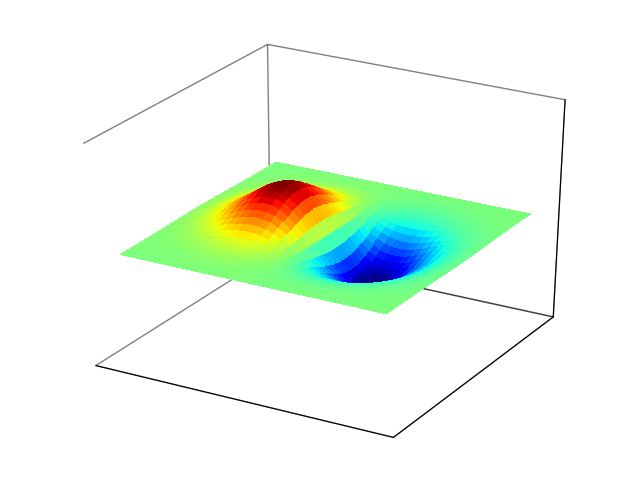
\includegraphics[width=0.14\textwidth]{Figures/LME_5_0_Shape_Fun_dx}\\
      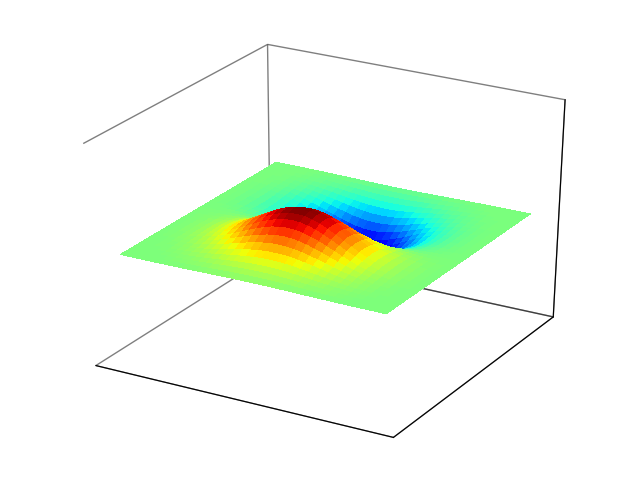
\includegraphics[width=0.14\textwidth]{Figures/LME_5_0_Shape_Fun_dy}
    \end{tabular}
  }
  \caption{Comparative of linear piecewise shape functions (Q4) and
    uniform GIMP shape functions (uGIMP) \textit{versus} Local max-ent
    shape functions for a two-dimensional arrangement of nodes, and
    spatial derivatives for several values of $\gamma = \beta/h^2$.}
  \label{fig:LME_MPM}
\end{figure*}
%%%%%%%%%%%%%%%%%%%%%%%%%%%%%%%%%%%%%%%%%%%%%%%%%%%%%%%%%%%%%%%%%%%%%%%%%%
In this research and in \cite{Arroyo2006}, $\Beta$ is a scalar as the
influence area of the shape function is controlled by the Euclidean
norm, therefore the search area is geometrically a circle in 2D, or a
sphere in 3D. Building upon the idea of anisotropic shape functions,
\cite{Kochmann2019} introduced an enhanced version of the original
local max-ent scheme, which uses an anisotropic support to deal with
tensile inestability. Nonetheless this is out of the scope of the
present document but will be incorporated in future research.

\section{Application to linear elasticity dynamic problems.}
\label{sec:Application-linear-elasticity-dynamic-problems}

This section is devoted to test the ability of both predictor-corrector
time integration scheme and the local \textit{max-ent} approximants to
overcome spurious oscillations due to the grid crossing and high
frequency loads under the context of MPM Two different test has
been adopted for this purpose, the benchmark proposed by Dyka \& Ingel
(1995)\cite{Dyka1995} and the test proposed in the PhD thesis of
Andersen (2009)\cite{thesis_Andersen_2009}. In all calculations we confine out attention to
uniformly distribute node and particle sets. The accuracy of the PCE
scheme is compared to the standard FE. In addition \textit{max-ent} solutions
are compared with those provided by uGIMP and Q4 shape functions, also
we compare MPM performance with OTM and FEM. All simulations were
performed with in-hose software. 

\subsection{Dyka bar}
\label{sec:dyka-bar}

This benchmark was proposed due to its ability to shows the capability
of the proposed time integration algorithm to avoid velocity
fields instabilities. It consists in a one-dimensional bar with a
length of 0.1333 meters, sketched in the
figure~\ref{fig:Dyka_Bar}. The boundary conditions are in the right
border displacement are constrained ($\vect{v} \rvert_{x=L} = 0$) and
in the left displacement are let free ($\tens{\sigma} \rvert_{x=0} =
0$). And a initial velocity of $\vect{v}_o = - 5\ m/s$ is given to the
last quarter of it. Finally, the elastic parameters consider for this test are:
\begin{itemize} 
\item  Density : $7833\ kg/m3$
\item  Poisson ratio : $0$
\item  Elastic modulus : $200 \cdot 10^9\ Pa$
\end{itemize}
%%%%%%%%%%%%%%%%%%%%%%%%%%%%%%%%%%%%%%%%%%%%%%%%%%%%%%%%%%%%%%%%%%%%%%%%%%
\begin{figure}\sidecaption
  \centering
  \resizebox{\hsize}{!}{
    \begin{tikzpicture} 
  \scaling{2}; 
  % Nodos 
  \point{a}{0}{1};
  \point{b}{3.75}{1};
  \point{c}{5}{1};
  % Barras
  \beam{2}{a}{b};
  \beam{2}{b}{c};
  % Apoyos
  \support{3}{a}[270];
  % Fuerzas
  \lineload{4}{b}{c}[1][0.2];
  \notation{5}{b}{c}[$5\ m/s$][.5][below][2];
  % Nombres de nodos
  \notation{1}{a}{A}[below right];
  \notation{1}{b}{B}[below right];
  \notation{1}{c}{C}[below right];
  % Cotas
  \dimensioning{1}{a}{b}{0.5}[{\unit[3/4]{L}}];
  \dimensioning{1}{b}{c}{0.5}[{\unit[1/4]{L}}];
\end{tikzpicture}
}
  \caption{Geometrical description of the Dyka \cite{Dyka1995} bar.}
  \label{fig:Dyka_Bar}
\end{figure}
%%%%%%%%%%%%%%%%%%%%%%%%%%%%%%%%%%%%%%%%%%%%%%%%%%%%%%%%%%%%%%%%%%%%%%%%%%
In this case a duration of 0.0001 seconds for the simulation is
consider. Therefore, the elastic wave generated travel thorough the bar
(from A to C and back to A) at least two times. For the spatial
discretization we propose a set a seven nodal mesh sizes (0.1, 0.3325, 0.5,
1.0, 3.3325, 6.665, 10.0) in millimeters. For each element a number of
four particles was selected. In the initial layout, particles are
occupying the exact quadrature points of a linear quadrilateral. With
the exception of the uGIMP simulation where gaps or overlap between
voxels of each particle are not allowed. In those cases, each particles
occupy the center of each cell quarter. For all simulations, time step
is controlled by a Courant-Friedrichs-Levy condition of 0.1, were the adopted
celerity is computed as,
\begin{equation}
  \label{eq:Cel}
  Cel = \max\{\max_{p \in \Omega_p}\{ \vect{v}_p \} , \max_{p \in \Omega_p}\{ \sqrt{\frac{E_p}{\rho_p}} \} \}
\end{equation}
A important consideration regarding modellization concerns to the
background mesh. Notice that free border of the bar has a maximum
horizontal displacement of 0.03 millimeters, therefore 
a computational domain with an extra gap of 0.03 millimeters is
required in order to accommodate the unconstrained displacement of the
particles in the left border of the bar. Naturally this problem arise
when the mesh size is small enough that relative displacement of the
particles are larger then the distance to the border, so grid crossing
phenomena could appear even in those cases with infinitesimal
displacements.
%%%%%%%%%%%%%%%%%%%%%%%%%%%%%%%%%%%%%%%%%%%%%%%%%%%%%%%%%%%%%%%%%%%%%%%%%% 
\begin{figure*}\sidecaption
  \centering
  \resizebox{0.7\hsize}{!}{
    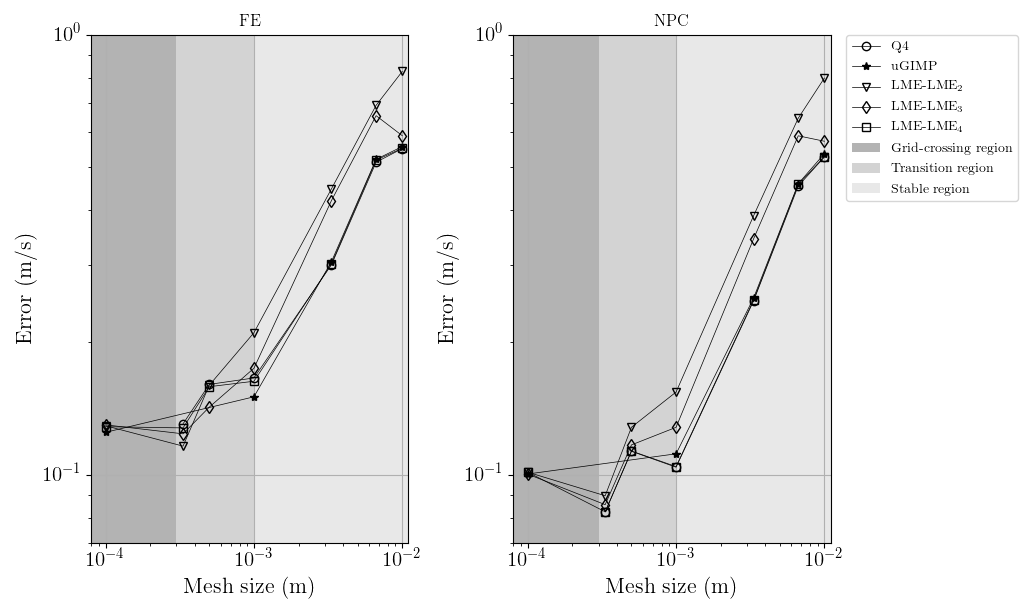
\includegraphics[width=\textwidth]{./Figures/Error_evol}
  }
  \caption{Velocity evolution at the point in the Dyka bar left side,
    convergence plots for FE and PCE. The plot is subdivided with
    colours, the darker part of the diagram shows coincides when the
    relative movement of the particles is large enough to produce the
    grid crossing phenomena. The lightest part of the diagram
    coincides when the relative movement of the particles in
    negligible in comparison with the mesh size. And in the middle
    region a transition behaviour take place.}
  \label{fig:Dyka-error-evol}
\end{figure*}
%%%%%%%%%%%%%%%%%%%%%%%%%%%%%%%%%%%%%%%%%%%%%%%%%%%%%%%%%%%%%%%%%%%%%%%%%%
In this case, an analytical solution is possible
thought the characteristics method described in the appendix
\ref{app:analytical_sol}. To measure the convergence of the solutions
for the different time integration and approximation schemes the
root-mean-square (RMS) error in the velocity field is computed. RMS
error is defined as
\begin{equation}
  \label{eq:RMS}
  RMS = \sqrt{\frac{1}{N} \sum^{N}_p \left( \vect{v}_p - \hat{\vect{v}}_p \right)^2},
\end{equation}
where $\vect{v}_p$ and $\hat{\vect{v}}_p$ are respectively the analytical and
numerical solutions evaluated in the final time step in the position
of each particle. A first comparative between both time integration
scheme is plotted in figure \ref{fig:Dyka-PCE-FE}. It demonstrates the
superior performance of the PCE \textit{versus} the FE. In the PCE the
spurious oscillations are quickly mitigated in the first time steps,
and does not propagate the error in time in opposite to FE where the
simulation becomes unstable after $6E^{5}$ seconds. Figure
\ref{fig:Dyka-error-evol} also remarks the remarkable difference
between both schemes. 
%%%%%%%%%%%%%%%%%%%%%%%%%%%%%%%%%%%%%%%%%%%%%%%%%%%%%%%%%%%%%%%%%%%%%%%%%%
\begin{figure}\sidecaption
  \centering
  \resizebox{0.9\hsize}{!}{
    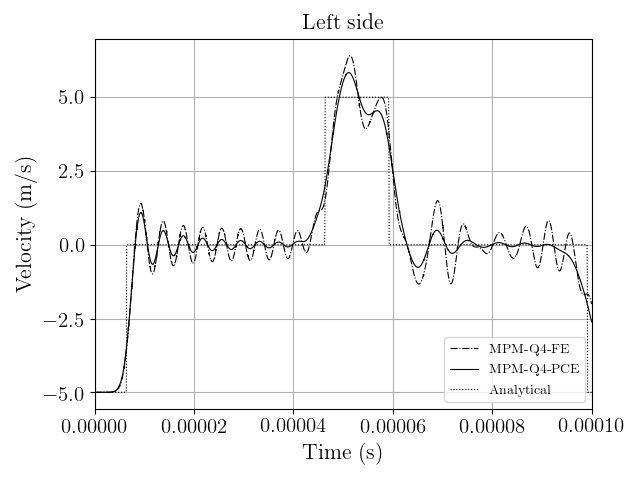
\includegraphics[width=\textwidth]{./Figures/Velocity_FE_vs_PCE_CFL_01}
  }
  \caption{Comparative of the PCE \textit{versus} the FE. In the
    picture the velocity evolution at the point in the bar left side
    is plotted.}
  \label{fig:Dyka-PCE-FE}
\end{figure}
%%%%%%%%%%%%%%%%%%%%%%%%%%%%%%%%%%%%%%%%%%%%%%%%%%%%%%%%%%%%%%%%%%%%%%%%%%
Figure \eqref{fig:Dyka-LME-gamma} shows the sensibility of the LME
approximation scheme to variations in the a-dimensional parameter
$\beta$ that controls the value of the regularization parameter
$\gamma$ depending of the mesh size. As we can see lower values of
gamma exhibits a behaviour with a soft decay in some parts of the
simulation due to the increase of nodes adopted to regularize the
solutions. This capability could be useful in simulations where
extremely noise oscillations could damage the solutions like memory
materials. On the other hand larger values of the parameter $\beta$
makes the solution tend to the linear FEM solution as the athermal
limit is reached \cite{Arroyo2006}. Intermediate values of the
regularization parameters give us a compromise between the both
scenarios here described. An additional observation concerning the
solution sensibility to regularization parameters occurs when mesh
size decreases. For larger mesh size where the relative particle displacement
is negligible in comparison with the cell size, the global behaviour
is FEM-like, therefore larger values of $\gamma$ has offers better
results. On the other hand, when mesh size is small enough to produce
grid-crossing and mesh-free behaviour is required to ensures the
convergence of the solution, tiny values of $\gamma$ has a better
performance. Convergence plot in figure \eqref{fig:Dyka-error-evol}
shows how the slope for the larger values of $\gamma$ decreases
monotonically with the value of the mesh size, in contrast to larger
values of it, whose suffers a punishment of the performance when significant
movement of the particles occurs as far we reduce the mesh size.  
%%%%%%%%%%%%%%%%%%%%%%%%%%%%%%%%%%%%%%%%%%%%%%%%%%%%%%%%%%%%%%%%%%%%%%%%%%
\begin{figure}\sidecaption
  \centering
  \resizebox{0.9\hsize}{!}{
    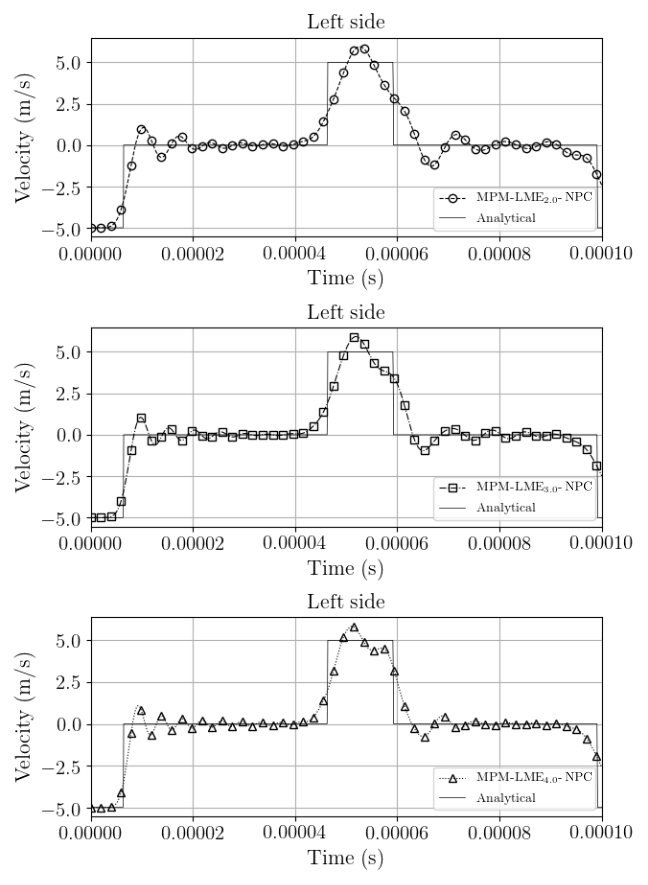
\includegraphics[width=\textwidth]{./Figures/Velocity_LME_gamma_comparative}
  }
  \caption{Sensitive of LME approximants performance to changes in the
    adimensional regularization parameter $\gamma = \beta/h^2$. To
    illustrate it, the velocity evolution at the point in the bar left side
    is plotted.}
  \label{fig:Dyka-LME-gamma}
\end{figure}
%%%%%%%%%%%%%%%%%%%%%%%%%%%%%%%%%%%%%%%%%%%%%%%%%%%%%%%%%%%%%%%%%%%%%%%%%%
Figure \ref{fig:Dyka-uGIMP-LME} compares the performance of the
uGIMP~\cite{Bardenhagen2004} shape function \textit{versus} the LME approximation scheme with
a adimensional regularization parameter $\gamma$ of 4.0. Although it
does not shows remarkable differences, LME approximats exhibits a more
robust behaviour than the uGIMP shape functions. Regarding this, notice
the absence of uGIMP values for a mesh size of 0.3325 and 0.5
millimeters. During these simulation the uGIMP suffered an unstable
increase of the error so we decided to no include this nodes in the
plot. A feasible explanation for this phenomena could be the presence
of numerical cancellation which could produce gaps between
voxels. Further research should be done in this direction for getting
a better comprehension of this phenomena. In opposite, LME
approximation does not suffers this phenomena either with irregular
nodal layout.
%%%%%%%%%%%%%%%%%%%%%%%%%%%%%%%%%%%%%%%%%%%%%%%%%%%%%%%%%%%%%%%%%%%%%%%%%%
\begin{figure}\sidecaption
  \centering
  \resizebox{0.9\hsize}{!}{
    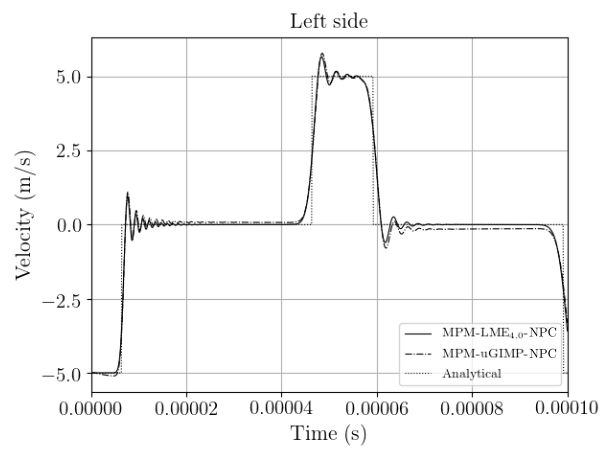
\includegraphics[width=\textwidth]{./Figures/Velocity_uGIMP_vs_LME_Dyka}
  }
  \caption{Velocity evolution at the point in the bar left side.}
  \label{fig:Dyka-uGIMP-LME}
\end{figure}
%%%%%%%%%%%%%%%%%%%%%%%%%%%%%%%%%%%%%%%%%%%%%%%%%%%%%%%%%%%%%%%%%%%%%%%%%%
Finally, figure \ref{fig:Dyka-OTM-MPM} compares the solution obtained
with OTM~\cite{Li2010} \textit{versus} the solution obtained with MPM,
both with same time integration scheme and spatial discretization. For
this case the performance of MPM is robust and stable than OTM. As we
can appreciate, during the first half of the simulation both method
seem to perform in a similar way, but during the second half of the
simulation after the elastic wave has travel from the free border to
the fixed one and back, in OTM the solution becomes noisy than the
one performed by MPM.  
%%%%%%%%%%%%%%%%%%%%%%%%%%%%%%%%%%%%%%%%%%%%%%%%%%%%%%%%%%%%%%%%%%%%%%%%%%
\begin{figure}\sidecaption
  \centering
  \resizebox{0.9\hsize}{!}{
    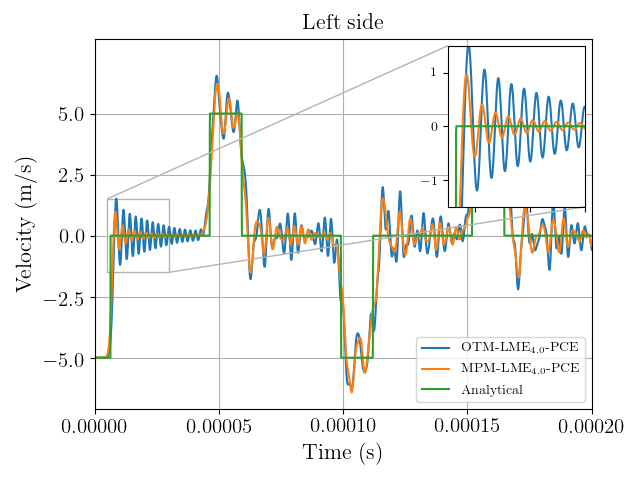
\includegraphics[width=\textwidth]{./Figures/Velocity_MPM_vs_OTM_Dyka}
  }
  \caption{Velocity evolution at the point in the bar left side.}
  \label{fig:Dyka-OTM-MPM}
\end{figure}
%%%%%%%%%%%%%%%%%%%%%%%%%%%%%%%%%%%%%%%%%%%%%%%%%%%%%%%%%%%%%%%%%%%%%%%%%%

\subsection{Andersen block}
\label{sec:andersen-block}

In order to test the ability of this interpolation technique to deal
with grid crossing instabilities we will simulate the vertical
compression of a square block (10 by 10 meters) of soft soil sketched
in figure~\ref{fig:block} and loaded using an incremental gravitation
scheme.
%%%%%%%%%%%%%%%%%%%%%%%%%%%%%%%%%%%%%%%%%%%%%%%%%%%%%%%%%%%%%%%%%%%%%%%%%%
\begin{figure}\sidecaption
  \centering
  \resizebox{0.7\hsize}{!}{
    \begin{tikzpicture} 
  \scaling{1};
  
% Nodos
\point{1}{0}{10};
\point{2}{2}{10};
\point{3}{0}{8};
\point{4}{2}{8};
\point{5}{4}{10};
\point{6}{0}{6};
\point{7}{2}{6};
\point{8}{4}{8};
\point{9}{4}{6};
\point{10}{6}{10};
\point{11}{0}{4};            
\point{12}{2}{4};            
\point{13}{6}{8};            
\point{14}{4}{4};            
\point{15}{6}{6};            
\point{16}{8}{10};            
\point{17}{0}{2};            
\point{18}{2}{2};            
\point{19}{8}{8};            
\point{20}{6}{4};            
\point{21}{4}{2};            
\point{22}{8}{6};            
\point{23}{0}{0};            
\point{24}{10}{10};            
\point{25}{6}{2};            
\point{26}{8}{4};
\point{27}{2}{0};            
\point{28}{10}{8};            
\point{29}{4}{0};            
\point{30}{10}{6};            
\point{31}{8}{2};            
\point{32}{6}{0};            
\point{33}{10}{4};            
\point{34}{8}{0};            
\point{35}{10}{2};            
\point{36}{10}{0};

% Barras
\beam{2}{27}{18};
\beam{2}{18}{17};
\beam{2}{17}{23};
\beam{2}{23}{27};
  
\beam{2}{29}{21};
\beam{2}{21}{18};
\beam{2}{18}{27};
\beam{2}{29}{27};

\beam{2}{32}{25};
\beam{2}{25}{21};
\beam{2}{21}{29};
\beam{2}{32}{29};

\beam{2}{34}{31};
\beam{2}{31}{25};
\beam{2}{25}{32};
\beam{2}{34}{32};

\beam{2}{36}{35};
\beam{2}{35}{31};
\beam{2}{31}{34};
\beam{2}{36}{34};

%%%%%%%%%%%%%%%%
\beam{2}{18}{12};
\beam{2}{12}{11};
\beam{2}{11}{17};
\beam{2}{18}{17};

\beam{2}{21}{14};
\beam{2}{14}{12};
\beam{2}{12}{18};
\beam{2}{21}{18};

\beam{2}{25}{20};
\beam{2}{20}{14};
\beam{2}{14}{21};
\beam{2}{25}{21};

\beam{2}{31}{26};
\beam{2}{26}{20};
\beam{2}{20}{25};
\beam{2}{31}{25};

\beam{2}{35}{33};
\beam{2}{33}{26};
\beam{2}{26}{31};
\beam{2}{35}{31};

%%%%%%%%%%%%%%%%
\beam{2}{12}{7};
\beam{2}{7}{6};
\beam{2}{6}{11};
\beam{2}{12}{11};

\beam{2}{14}{9};
\beam{2}{9}{7};
\beam{2}{7}{12};
\beam{2}{14}{12};

\beam{2}{20}{15};
\beam{2}{15}{9};
\beam{2}{9}{14};
\beam{2}{20}{14};

\beam{2}{26}{22};
\beam{2}{22}{15};
\beam{2}{15}{20};
\beam{2}{26}{20};

\beam{2}{33}{30};
\beam{2}{30}{22};
\beam{2}{22}{26};
\beam{2}{33}{26};

%%%%%%%%%%%%%%%%
\beam{2}{7}{4};
\beam{2}{4}{3};
\beam{2}{3}{6};
\beam{2}{7}{6};

\beam{2}{9}{8};
\beam{2}{8}{4};
\beam{2}{4}{7};
\beam{2}{9}{7};

\beam{2}{15}{13};
\beam{2}{13}{8};
\beam{2}{8}{9};
\beam{2}{15}{9};

\beam{2}{22}{19};
\beam{2}{19}{13};
\beam{2}{13}{15};
\beam{2}{22}{15};

\beam{2}{30}{28};
\beam{2}{28}{19};
\beam{2}{19}{22};
\beam{2}{30}{22};

%%%%%%%%%%%%%%%%
\beam{2}{4}{2};
\beam{2}{2}{1};
\beam{2}{1}{3};
\beam{2}{4}{3};

\beam{2}{8}{5};
\beam{2}{5}{2};
\beam{2}{2}{4};
\beam{2}{8}{4};

\beam{2}{13}{10};
\beam{2}{10}{5};
\beam{2}{5}{8};
\beam{2}{13}{8};

\beam{2}{19}{16};
\beam{2}{16}{10};
\beam{2}{10}{13};
\beam{2}{19}{13};

\beam{2}{28}{24};
\beam{2}{24}{16};
\beam{2}{16}{19};
\beam{2}{28}{19};

% Bottom
\support {1}{23}[315];
\support {1}{27}[0];
\support {1}{29}[0];
\support {1}{32}[0];
\support {1}{34}[0];
\support {1}{36}[45];

% \support {2}{23}[270];
\support {2}{1}[270];
\support {2}{3}[270];
\support {2}{6}[270];
\support {2}{11}[270];
\support {2}{17}[270];

\support {2}{24}[90];
\support {2}{28}[90];
\support {2}{30}[90];
\support {2}{33}[90];
\support {2}{35}[90];
% \support {2}{36}[90];

% Gravity
\point{g}{12}{5};
\load{1}{g}[90][3][0];

% Cotas
\dimensioning{1}{23}{36}{-1.5}[$10~m$];
\dimensioning{2}{23}{1}{-1.5}[$10~m$];


\end{tikzpicture}


% % Apoyos
% \support{3}{c}[90];
% % Fuerzas
% \lineload{4}{b}{a}[1][0.2];
% \notation{5}{a}{b}[$-5\ m/s$][.5][below][2];
% % Nombres de nodos
% \notation{1}{a}{A}[below left];
% \notation{1}{b}{B}[below left];
% \notation{1}{c}{C}[below left];
% % Cotas
% \dimensioning{1}{a}{b}{0.5}[{\unit[1/4]{L}}];
% \dimensioning{1}{b}{c}{0.5}[{\unit[3/4]{L}}];


% End Elements
}
  \caption{Geometrical description of a soil block }.}
  \label{fig:block}
\end{figure}
%%%%%%%%%%%%%%%%%%%%%%%%%%%%%%%%%%%%%%%%%%%%%%%%%%%%%%%%%%%%%%%%%%%%%%%%%%
This test was taken from PhD thesis of Andersen (2009)\cite{thesis_Andersen_2009}. The
elastic parameters consider for this test are: 
\begin{itemize} 
\item  Initial density : $6\cdot 10^3\ kg/m^3$
\item  Poisson ratio : $0$
\item  Elastic modulus : $5\ MPa$
\end{itemize}
The gravity force is a apply as an external force according to the
equations \eqref{eq:particle_body_forces},
\eqref{eq:nodal_external_forces}. Using a total time period of T (20
seconds) to apply the gravity, it is increased from 0 to 9.81$m/s$
with a sinus function until T/2 and then maintained constant until T
in order to arrive to a state of equilibrium, 
\begin{equation}
  \label{eq:gravity-load-block}
 \mathbf{g}(t) = \left\{
    \begin{array}{ll}
      0.5 \mathbf{g} (\sin(\frac{2t \pi}{T} - \frac{\pi}{2})+1)  & \mbox{if } t \leq T/2 \\
      \mathbf{g} & \mbox{if } t > T/2
    \end{array}
  \right.
\end{equation}
In order to get a stable solution, we will adopt a time step conducted
by a Courant number of 0.1. On the other hand, the explicit predictor-corrector
scheme is here employed looking forward getting better results. For the
initial spatial discretization we will employ four particles per cell
($\Delta x = 2\ m$). The initial setting of particles inside of the
cell changes according to the approximation technique adopted. For the
bi-linear shape functions and the LME approximants, the initial
position corresponds to the location of the gauss-points in a standard
quadratic finite element. For the uGIMP shape function the initial
position of each particle is located in the center of each voxel, due
to the fact that in the initial situation, the voxel domain should not
overlap each others.

Figure~\ref{fig:Block-LME3} shows the evolution of the vertical stress
during the loading process. The result is physically realistic as
stress increments linearly from the top to the bottom of the specimen,
and the value of the vertical stress in a material point located in
the bottom of the specimen oscillates centered in $5.2 MPa$, which is
the analytic value given by $\sigma_{yy} = \rho g h_y$.
%%%%%%%%%%%%%%%%%%%%%%%%%%%%%%%%%%%%%%%%%%%%%%%%%%%%%%%%%%%%%%%%%%%%%%%%%%
\begin{figure*}
  \centering
  \subfigure[t = 0 seconds.]{
    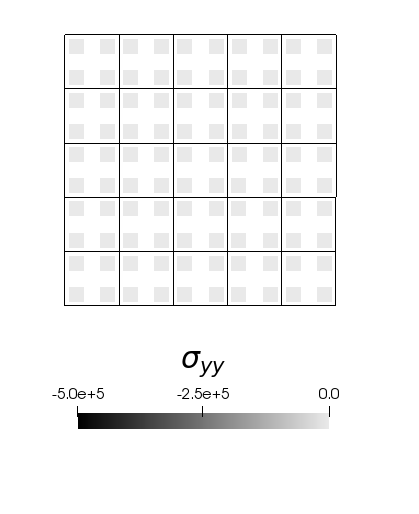
\includegraphics[width=0.32\textwidth]{Figures/Block_LME3_PCE_a_t0}
  }
  \subfigure[t = 5 seconds.]{
    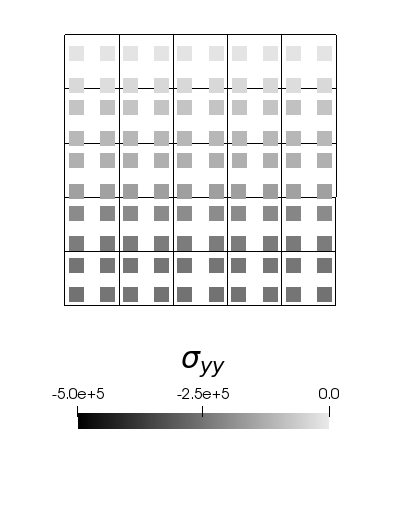
\includegraphics[width=0.32\textwidth]{Figures/Block_LME3_PCE_b_t025}
  }
  \subfigure[t = 20 seconds]{
    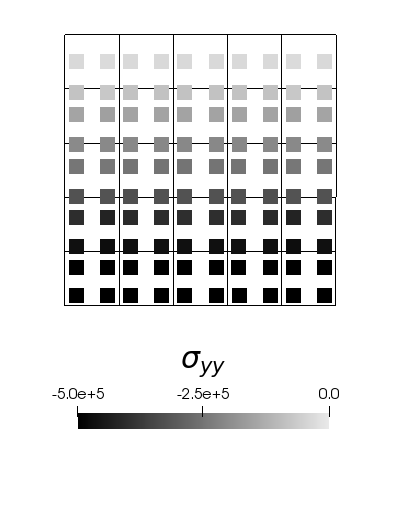
\includegraphics[width=0.32\textwidth]{Figures/Block_LME3_PCE_c_t1}
  }
  \caption{Vertical normal stress and position of material points
    during the loading process for a soft soil ($E = 5\ MPa$, $\rho_0
    = 6\cdot 10^3\ kg/m^3$). Numerical parameters considered for the
    simulation are : Local \textit{max-ent} shape function $\gamma =3$
    and explicit PC scheme with CFL 0.1.}
  \label{fig:Block-LME3}
\end{figure*}
%%%%%%%%%%%%%%%%%%%%%%%%%%%%%%%%%%%%%%%%%%%%%%%%%%%%%%%%%%%%%%%%%%%%%%%%%%
Figure~\ref{fig:vertical-displacement-block} shows the vertical
displacement evolution of a point in the free surface of the block. As
we can see the simulation using the Q4 interpolation technique turns
out to be unstable and in the second 15 it fails. The uGIMP simulation
is more stable than the one performed by the Q4. Despite this is still
unstable and could trigger severe oscillations if we pretend to
simulate non-linear materials. The LME simulation was performed using
two kinds of shape functions, one with a low value of the
dimensionless parameter, $\gamma = 0.8$, and other with a larger value
of it, $\gamma = 3.0$. Notice that the results are both stable, but
the larger values of $\gamma$ give us a very stable solution. This is
due to the fact that with larger value of $\gamma$, the shape
functions behaves in a similar way to the FEM, which performs very
accurate in those cases with a reasonable mesh distorsion, and with a
lower value it behaves in a similar way to the uGIMP. This behaviour
was noticed previously by \cite{Arroyo2006}, were authors highlight
how by adjusting the spatial variation of $\beta(\vect{x})$, it is
possible to select regions of the domain of analysis which are treated
by finite elements and regions that are treated in the style of
meshfree methods, with seamless transitions between those regions. 
%%%%%%%%%%%%%%%%%%%%%%%%%%%%%%%%%%%%%%%%%%%%%%%%%%%%%%%%%%%%%%%%%%%%%%%%%%
\begin{figure}\sidecaption
  \centering
  \resizebox{\hsize}{!}{
    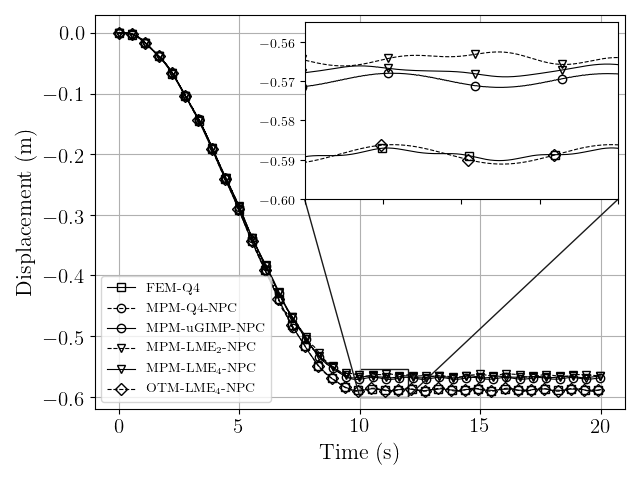
\includegraphics[width=\textwidth]{./Figures/Block_CFL_01_Comparative}
  }
  \caption{Comparative of the vertical displacement evolution in a
    point located in the free surface employing different
    interpolation schemes and numerical techniques.} 
  \label{fig:vertical-displacement-block}
\end{figure}
%%%%%%%%%%%%%%%%%%%%%%%%%%%%%%%%%%%%%%%%%%%%%%%%%%%%%%%%%%%%%%%%%%%%%%%%%%


\section{Conclusions}
\label{sec:conclusions}
We have developed a novel time integration scheme for MPM, and
proved how local \textit{max-ent} approximation scheme could be
employed as an useful technique in MPM. The PCE arise as a highly
efficient alternative for challenging dynamic problems like coupled
$u-p_w$ without appeal to expensive implicit time integration
algorithms. Also the procedure employed to design the PCE algorithm open
the door to revisit a huge variety of time integration schemes
developed originally for FEM, which can be rearranged to MPM framework
with some modifications. Anyway, further research should be done to improve the
formal comprehension of the algorithm good performance. This paper
also enhances the suitability of the local \textit{max-ent} as a
general promising alternative to the wide range of approximation.
techniques developed for the MPM to overcome grid crossing
limitations and to avoid the constriction of the uGIMP of a regular mesh
or a high density of particles per cell. Future research of the
group will be on the employ of this scheme to improve the localization
capabilities of MPM for viscoplastic materials. Finally we remark on
the possibility of adapting the function $\beta(\vect{x})$ as a second
order tensor with the aim of adapt the shape function with the strain field which improves the
performance of it in the aforementioned localization
capabilities. Other possibility is to adapt the value of $\beta$ to
solve the equations fem-like of meshfree-like depending of how behaves
the region, this could be extremely useful in simulating all together
initialization and propagation of fast landslides.

\begin{acknowledgements}
If you'd like to thank anyone, place your comments here
and remove the percent signs.
\end{acknowledgements}

%
\section*{Conflict of interest}
%
The authors declare that they have no conflict of interest.

\appendix

\section{The analytical solution of the 1D Dyka benchmark}
\label{app:analytical_sol}

For the derivation of this analytical solution we will consider  the
dynamic behaviour of a 1D elastic bar. The governing equations are the
following: (i) The balance of linear momentum,
\begin{equation}
  \label{eq:1D-balance-linear-momentum}
  \rho\ \Deriv{v}{t} = \Deriv{\sigma}{x},
\end{equation}
where $\sigma$ is the stress value, $\rho$ is the density, and 
$v$ is the velocity. (ii) The constitutive model, which for convenience of the
following developments will be written in terms of displacement and
velocities as, 
\begin{equation}
  \label{eq:1D-constitutive-equation}
  \Deriv{\sigma}{t} = E \Deriv{\varepsilon}{t},
\end{equation}
where $E$ is the elastic modulus. (iii) The compatibility equation
also in terms of the velocity field,
\begin{equation}
  \label{eq:CompatibilityEquation_e}
  \Deriv{\varepsilon}{t} = \Deriv{v}{x}.
\end{equation}
Next for simplicity, we will introduce \eqref{eq:CompatibilityEquation_e} in 
\eqref{eq:1D-constitutive-equation}, so we get the following system of equations,
\begin{align}
  \label{eq:1D-balance-linear-momentum-II}
  \Deriv{v}{t} &= \frac{1}{\rho}\ \Deriv{\sigma}{x}, \\
  \label{eq:1D-constitutive-equation-II}
  \Deriv{\sigma}{t} &= E\ \Deriv{v}{x}.
\end{align}

Introducing \eqref{eq:1D-constitutive-equation-II} in
\eqref{eq:1D-balance-linear-momentum-II} and expressing the remaining
equation in terms of the displacement, we reach the 1D wave
equation for linear elastic materials,
\begin{equation}
  \label{eq:1D-wave-elastic}
  \Deriv[2]{u}{t} = \frac{E}{\rho}\ \Deriv[2]{u}{x} = c^2\ \Deriv[2]{u}{x}
\end{equation}
where we have introduced the wave celerity $c$ as,
\begin{equation}
  \label{eq:1D-elastic-wave-celerity}
  c = \sqrt{\frac{E}{\rho}}
\end{equation}
Alternative, rearranging both equations
\eqref{eq:1D-balance-linear-momentum-II} and
\eqref{eq:1D-constitutive-equation-II} it is possible to join them in a
single system of equations as,
\begin{equation}
  \label{eq:System-stress-velocity}
  \Deriv{}{t} \left[
    \begin{array}{c}
      \sigma \\
      v
    \end{array}
  \right] + \left[
    \begin{array}{cc}
      0 & - E \\
      - 1/\rho & 0 
    \end{array} \right] \left[
    \begin{array}{c}
      \Deriv{\sigma}{x} \\
      \Deriv{v}{x}
    \end{array}
  \right] = \Vector{0}.
\end{equation}
This expression can be written in a more compact format as,
\begin{equation}
  \label{eq:System-stress-velocity-II}
  \Deriv{\Vector{\phi}}{t} + \Matrix{A}\Deriv{\Vector{\phi}}{x} = \Vector{0}
\end{equation}
where both variables are joined in a single vectorial variable
$\Vector{\phi}$ and $\Matrix{A}$ in coupling matrix between both equations,
\begin{equation*}
  \Vector{\phi} = \left[
    \begin{array}{c}
      \sigma \\
      v
    \end{array}
  \right],\quad 
  \Matrix{A} =  \left[
    \begin{array}{cc}
      0 & - E\\
      - 1/\rho & 0 
    \end{array} \right].
\end{equation*}
Note that the nature of \label{eq:eq:System-stress-velocity-II} is still
hyperbolic despite the fact it does not have a second order
temporal derivative as \eqref{eq:1D-wave-elastic}. A proof of this can
be easily obtained if we get the zeros of the hypersurface defined by
\eqref{eq:1D-wave-elastic}. And later the eigenvalues of $\Matrix{A}$
in \eqref{eq:System-stress-velocity-II}. In both cases, eigenvalues
are real and distinct ($\lambda = \pm \sqrt{\frac{E}{\rho}}$),
therefore the system is called strictly hyperbolic.

For a more general description in the following, we will assume that $\Matrix{A}$ has $n$
different eigenvalues $\{ \lambda_1, \lambda_2, \ldots, \lambda_i, \ldots
\lambda_n \}$ and $n$ eigenvectors $\{ \vec{x}^1, \vec{x}^2, \ldots,
\vec{x}^i, \ldots \vec{x}^n \}$ satisfying that $\tens{A} \vec{x} =
\lambda \vec{x} $. Now we introduce the matrix $\Matrix{P}$ whose columns are the $n$
eigenvalues $\Vector{x}$
\begin{equation}
  \label{eq:P-matrix}
\Matrix{P} = \{ \vec{x}^1, \vec{x}^2, \vec{x}^3, \ldots \vec{x}^n \}.
\end{equation}
Diagonalizing $\Matrix{A}$ using $\Matrix{P}$ we get
\begin{equation}
  \label{eq:Lambda-matrix}
  \Lambda = \Matrix{P}^{-1} \Matrix{A}\ \Matrix{P},
\end{equation}
where $ \Lambda_{ii} = \lambda_i$. Next we will define a vector $\Vector{\Re}$ such that:
\begin{equation}
  \label{eq:Riemann-definition}
  \Vector{\phi} = \Matrix{P}\ \Vector{\Re}
\end{equation}
we will assume to be integrable. Expanding the above expression with
the chain rule and passing the matrix $\Matrix{P}$ to left hand side
of the equality we get,
\begin{equation}
  \label{eq:Riemann-II}
  d \vec{\Vector{\Re}} = \Deriv{\Vector{\Re}}{t}dt + \Deriv{\Vector{\Re}}{x}dx =
  \tens{P}^{-1}\left(\Deriv{\phi}{t}dt + \Deriv{\phi}{x}dx \right)
\end{equation}
and setting the terms we get,
\begin{equation}
  \label{eq:Riemann-III}
  \Deriv{\Vector{\Re}}{t} = \Matrix{P}^{-1}\Deriv{\Vector{\phi}}{t},\quad 
  \Deriv{\Vector{\Re}}{x} = \Matrix{P}^{-1}\Deriv{\Vector{\phi}}{x}
\end{equation}
Next, if we multiply \eqref{eq:System-stress-velocity-II} by
$\Matrix{P}^{-1}$ we get:
\begin{equation}
  \label{eq:System-stress-velocity-III}
  \Matrix{P}^{-1}\Deriv{\Vector{\phi}}{t} + \left(\Matrix{P}^{-1}\Matrix{A}\Matrix{P}
  \right)\Matrix{P}^{-1} \Deriv{\Vector{\phi}}{x} = \Vector{0}
\end{equation}
finally introducing the expressions \eqref{eq:Riemann-III} we reach to
\begin{equation}
  \label{eq:System-stress-velocity-IV}
  \Deriv{\Vector{\Re}}{t} + \varLambda \Deriv{\Vector{\Re}}{x} = \Vector{0}  
\end{equation}
which consists of $n$ uncoupled equations as $\varLambda$ is
diagonal matrix as we can see in \eqref{eq:Lambda-matrix}. Each of this
equations are 1D scalar convective transport equations, with solutions
of the form:
\begin{equation}
  \label{eq:SystemEquations_sigma_v_VI}
  \Re^{(i)} = F^{(i)} \left(x - \lambda^{(i)} t \right)
\end{equation}

This uncoupled system, has, therefore, a set of $n$ characteristics.
These magnitudes $\Re_i$ which propagate along characteristics are
known as ``Riemann invariants'' of the problem. Here we have a 1D
configuration, so the domain is $\Omega : \left(0, L\right) x \left(0,
  T\right)$. For the closure of the problem we require:
\begin{itemize}
\item ``n'' initial conditions of the form $\Re_i (x,t=0) = h_i(x)$,
  where $i = {0, \ldots, n}$, and $h_i(x)$ is a vectorial function
  given by the physical variables of the problem.
\item ``n'' boundary conditions.
\end{itemize}

Now particularizing the previous equations for the 1D elastic bar
described in \cite{Dyka1995}, we get that the matrix $\Matrix{P}$
is the following:
\begin{equation*}
    \Matrix{P} =  \left[
    \begin{array}{cc}
      -\sqrt{E\rho} & \sqrt{E\rho}\\
       1 & 1 
    \end{array} \right]
\end{equation*}
and its inverse is:
\begin{equation*}
    \Matrix{P}^{-1} = \frac{1}{2\ \sqrt{E\rho}} \left[
    \begin{array}{cc}
      -1 & \frac{1}{\sqrt{E\rho}}\\
      1 & \frac{1}{\sqrt{E\rho}} 
    \end{array} \right]
\end{equation*}

And introducing the value of the inverse matrix $\Matrix{P}^1$ in the
Riemann definition \eqref{eq:Riemann-definition} we get the following
system of equations,
\begin{align}
  \label{eq:Riemann-I-1D-elastic-bar}
  &\Re^{I} = \frac{1}{2\sqrt{\rho E}}\left(-\sigma + v\ \sqrt{\rho E}
    \right)\\
  \label{eq:Riemann-II-1D-elastic-bar}
  &\Re^{II} = \frac{1}{2\sqrt{\rho E}}\left(\sigma + v\ \sqrt{\rho E} \right)
\end{align}

From \eqref{eq:Riemann-I-1D-elastic-bar} and
\eqref{eq:Riemann-II-1D-elastic-bar} we can obtain the values of the
stress and the velocity as:
\begin{equation}
  \label{eq:Riemann-stress-velocity}
  v = \Re^{I} + \Re^{II} \quad , \quad \sigma = \sqrt{E \rho}\left(\Re^{II} - \Re^{I} \right)
\end{equation}

The boundary conditions are in both cases of radiation as there is not
wave in-going from the exterior. So for the right side (fixed
boundary) we get the following conditions:
\begin{equation*}
  \Re^{II} = 0 \quad and \quad v_{x=L} = 0
\end{equation*}
Therefore $\sigma_{x=L} = -2\sqrt{\rho E}\ \Re^{I}$. And in the left side
(free boundary) we get the following conditions:
\begin{equation*}
  \Re^{I} = 0 \quad and \quad \sigma_{x=0} = 0
\end{equation*}
Therefore $v_{x=0} = 2\Re^{II}$. Finally, applying this conditions in
the elastic bar sketched in figure~\ref{fig:Dyka_Bar}, is possible to obtain
the velocity history in the right side of the bar plotted in the figure~\ref{fig:vel_analytics_dyka} and the stress in the last quarter side of the Dyka
bar plotted in the figure~\ref{fig:stress_analytics_dyka} as is demanded in \cite{Dyka1995}.

\begin{figure}\sidecaption
  \centering
  \resizebox{\hsize}{!}{
    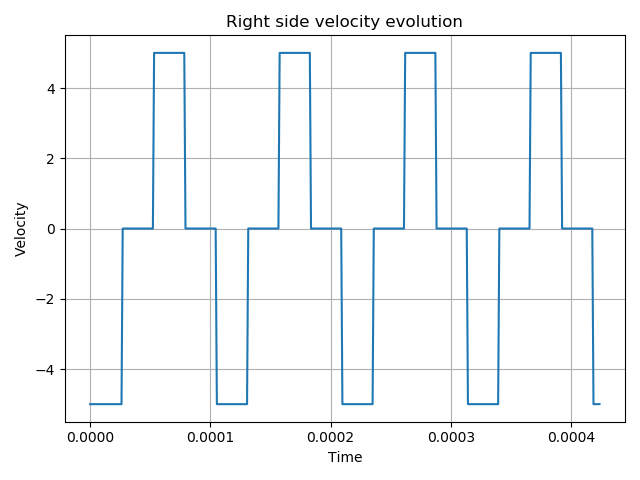
\includegraphics[width=\columnwidth]{Figures/1D_right_Velocity.png}
  }
  \caption[Velocities values in the right side of the Dyka
  bar]{Analytical solution for the velocity in the right side of the Dyka bar.}
  \label{fig:vel_analytics_dyka}
\end{figure}

\begin{figure}\sidecaption
  \centering
  \resizebox{\hsize}{!}{
    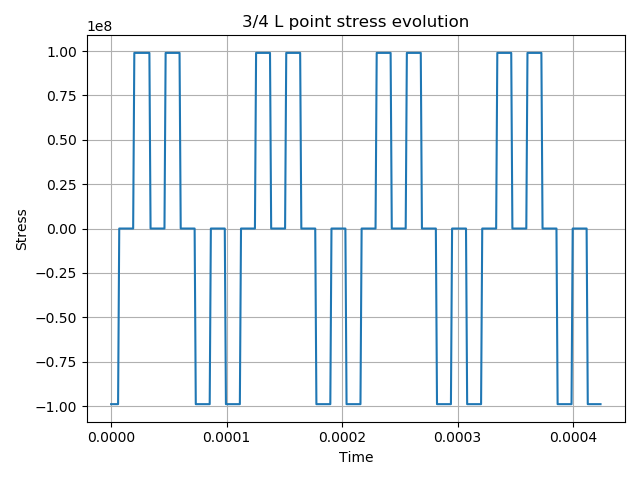
\includegraphics[width=\columnwidth]{Figures/1D_left_Stress.png}
  }
  \caption[Stress values in the last quarter side of the Dyka
  bar]{Analytical solution for the stress in the last quarter of the Dyka bar.}
  \label{fig:stress_analytics_dyka}
\end{figure}



% BibTeX users please use one of
%\bibliographystyle{spbasic}      % basic style, author-year citations
\bibliographystyle{spmpsci}      % mathematics and physical sciences
%\bibliographystyle{spphys}       % APS-like style for physics
\bibliography{Biblio}   % name your BibTeX data base

\end{document}
% end of file template.tex


%%% Local Variables:
%%% mode: latex
%%% TeX-master: t
%%% End:

